% Options for packages loaded elsewhere
\PassOptionsToPackage{unicode}{hyperref}
\PassOptionsToPackage{hyphens}{url}
%
\documentclass[
  8pt,
  ignorenonframetext,
]{beamer}
\usepackage{pgfpages}
\setbeamertemplate{caption}[numbered]
\setbeamertemplate{caption label separator}{: }
\setbeamercolor{caption name}{fg=normal text.fg}
\beamertemplatenavigationsymbolsempty
% Prevent slide breaks in the middle of a paragraph
\widowpenalties 1 10000
\raggedbottom
\setbeamertemplate{part page}{
  \centering
  \begin{beamercolorbox}[sep=16pt,center]{part title}
    \usebeamerfont{part title}\insertpart\par
  \end{beamercolorbox}
}
\setbeamertemplate{section page}{
  \centering
  \begin{beamercolorbox}[sep=12pt,center]{part title}
    \usebeamerfont{section title}\insertsection\par
  \end{beamercolorbox}
}
\setbeamertemplate{subsection page}{
  \centering
  \begin{beamercolorbox}[sep=8pt,center]{part title}
    \usebeamerfont{subsection title}\insertsubsection\par
  \end{beamercolorbox}
}
\AtBeginPart{
  \frame{\partpage}
}
\AtBeginSection{
  \ifbibliography
  \else
    \frame{\sectionpage}
  \fi
}
\AtBeginSubsection{
  \frame{\subsectionpage}
}
\usepackage{amsmath,amssymb}
\usepackage{lmodern}
\usepackage{ifxetex,ifluatex}
\ifnum 0\ifxetex 1\fi\ifluatex 1\fi=0 % if pdftex
  \usepackage[T1]{fontenc}
  \usepackage[utf8]{inputenc}
  \usepackage{textcomp} % provide euro and other symbols
\else % if luatex or xetex
  \usepackage{unicode-math}
  \defaultfontfeatures{Scale=MatchLowercase}
  \defaultfontfeatures[\rmfamily]{Ligatures=TeX,Scale=1}
\fi
% Use upquote if available, for straight quotes in verbatim environments
\IfFileExists{upquote.sty}{\usepackage{upquote}}{}
\IfFileExists{microtype.sty}{% use microtype if available
  \usepackage[]{microtype}
  \UseMicrotypeSet[protrusion]{basicmath} % disable protrusion for tt fonts
}{}
\makeatletter
\@ifundefined{KOMAClassName}{% if non-KOMA class
  \IfFileExists{parskip.sty}{%
    \usepackage{parskip}
  }{% else
    \setlength{\parindent}{0pt}
    \setlength{\parskip}{6pt plus 2pt minus 1pt}}
}{% if KOMA class
  \KOMAoptions{parskip=half}}
\makeatother
\usepackage{xcolor}
\IfFileExists{xurl.sty}{\usepackage{xurl}}{} % add URL line breaks if available
\IfFileExists{bookmark.sty}{\usepackage{bookmark}}{\usepackage{hyperref}}
\hypersetup{
  hidelinks,
  pdfcreator={LaTeX via pandoc}}
\urlstyle{same} % disable monospaced font for URLs
\newif\ifbibliography
\usepackage{color}
\usepackage{fancyvrb}
\newcommand{\VerbBar}{|}
\newcommand{\VERB}{\Verb[commandchars=\\\{\}]}
\DefineVerbatimEnvironment{Highlighting}{Verbatim}{commandchars=\\\{\}}
% Add ',fontsize=\small' for more characters per line
\usepackage{framed}
\definecolor{shadecolor}{RGB}{248,248,248}
\newenvironment{Shaded}{\begin{snugshade}}{\end{snugshade}}
\newcommand{\AlertTok}[1]{\textcolor[rgb]{0.94,0.16,0.16}{#1}}
\newcommand{\AnnotationTok}[1]{\textcolor[rgb]{0.56,0.35,0.01}{\textbf{\textit{#1}}}}
\newcommand{\AttributeTok}[1]{\textcolor[rgb]{0.77,0.63,0.00}{#1}}
\newcommand{\BaseNTok}[1]{\textcolor[rgb]{0.00,0.00,0.81}{#1}}
\newcommand{\BuiltInTok}[1]{#1}
\newcommand{\CharTok}[1]{\textcolor[rgb]{0.31,0.60,0.02}{#1}}
\newcommand{\CommentTok}[1]{\textcolor[rgb]{0.56,0.35,0.01}{\textit{#1}}}
\newcommand{\CommentVarTok}[1]{\textcolor[rgb]{0.56,0.35,0.01}{\textbf{\textit{#1}}}}
\newcommand{\ConstantTok}[1]{\textcolor[rgb]{0.00,0.00,0.00}{#1}}
\newcommand{\ControlFlowTok}[1]{\textcolor[rgb]{0.13,0.29,0.53}{\textbf{#1}}}
\newcommand{\DataTypeTok}[1]{\textcolor[rgb]{0.13,0.29,0.53}{#1}}
\newcommand{\DecValTok}[1]{\textcolor[rgb]{0.00,0.00,0.81}{#1}}
\newcommand{\DocumentationTok}[1]{\textcolor[rgb]{0.56,0.35,0.01}{\textbf{\textit{#1}}}}
\newcommand{\ErrorTok}[1]{\textcolor[rgb]{0.64,0.00,0.00}{\textbf{#1}}}
\newcommand{\ExtensionTok}[1]{#1}
\newcommand{\FloatTok}[1]{\textcolor[rgb]{0.00,0.00,0.81}{#1}}
\newcommand{\FunctionTok}[1]{\textcolor[rgb]{0.00,0.00,0.00}{#1}}
\newcommand{\ImportTok}[1]{#1}
\newcommand{\InformationTok}[1]{\textcolor[rgb]{0.56,0.35,0.01}{\textbf{\textit{#1}}}}
\newcommand{\KeywordTok}[1]{\textcolor[rgb]{0.13,0.29,0.53}{\textbf{#1}}}
\newcommand{\NormalTok}[1]{#1}
\newcommand{\OperatorTok}[1]{\textcolor[rgb]{0.81,0.36,0.00}{\textbf{#1}}}
\newcommand{\OtherTok}[1]{\textcolor[rgb]{0.56,0.35,0.01}{#1}}
\newcommand{\PreprocessorTok}[1]{\textcolor[rgb]{0.56,0.35,0.01}{\textit{#1}}}
\newcommand{\RegionMarkerTok}[1]{#1}
\newcommand{\SpecialCharTok}[1]{\textcolor[rgb]{0.00,0.00,0.00}{#1}}
\newcommand{\SpecialStringTok}[1]{\textcolor[rgb]{0.31,0.60,0.02}{#1}}
\newcommand{\StringTok}[1]{\textcolor[rgb]{0.31,0.60,0.02}{#1}}
\newcommand{\VariableTok}[1]{\textcolor[rgb]{0.00,0.00,0.00}{#1}}
\newcommand{\VerbatimStringTok}[1]{\textcolor[rgb]{0.31,0.60,0.02}{#1}}
\newcommand{\WarningTok}[1]{\textcolor[rgb]{0.56,0.35,0.01}{\textbf{\textit{#1}}}}
\usepackage{longtable,booktabs,array}
\usepackage{calc} % for calculating minipage widths
\usepackage{caption}
% Make caption package work with longtable
\makeatletter
\def\fnum@table{\tablename~\thetable}
\makeatother
\setlength{\emergencystretch}{3em} % prevent overfull lines
\providecommand{\tightlist}{%
  \setlength{\itemsep}{0pt}\setlength{\parskip}{0pt}}
\setcounter{secnumdepth}{-\maxdimen} % remove section numbering
% type setting
% ------------------------------------------------------------------------------
\usepackage[german]{babel}     

% fonts
% ------------------------------------------------------------------------------
\usefonttheme{professionalfonts}

% slide title and horizontal line
% ------------------------------------------------------------------------------
\setbeamertemplate{frametitle}{%
    \vskip-30pt \color{black}\large%
    \begin{minipage}[b][23pt]{120mm}%
    \flushleft\insertframetitle%
    \end{minipage}%
}

\setbeamertemplate{headline}										
{
\vskip10pt\hfill\hspace{3.5mm} 										 
\vskip15pt\color{black}\rule{\textwidth}{0.4pt} 					 
}

% slide number
% ---------------------------------------------------------------
\setbeamertemplate{navigation symbols}{}
\setbeamertemplate{footline}
{
\vskip5pt
\vskip2pt
\makebox[123mm]{\hspace{7.5mm}
\hfill Allgemeines Lineares Modell $\vert$ 
\copyright $ $ 2022 Dirk Ostwald CC BY-NC-SA 4.0 $\vert$ 
Folie \insertframenumber}
\vskip4pt
}

% block color scheme
% ------------------------------------------------------------------------------
% colors
\definecolor{white}{RGB}{255,255,255}
\definecolor{grey}{RGB}{235,235,235}
\definecolor{lightgrey}{RGB}{245,245,245}
\definecolor{LightBlue}{RGB}{220,220,255}
\definecolor{darkblue}{RGB}{51, 51, 153}

% definitions and theorems
\setbeamercolor{block title}{fg = black, bg = grey}
\setbeamercolor{block body}{fg = black, bg = lightgrey}

% general line spacing 
% ------------------------------------------------------------------------------
\linespread{1.3}

% local line spacing
% ------------------------------------------------------------------------------
\usepackage{setspace}

% colors
% -----------------------------------------------------------------------------
\usepackage{color}

% justified text
% ------------------------------------------------------------------------------
\usepackage{ragged2e}
\usepackage{etoolbox}
\apptocmd{\frame}{}{\justifying}{}

% bullet point lists
% -----------------------------------------------------------------------------
\setbeamertemplate{itemize item}[circle]
\setbeamertemplate{itemize subitem}[circle]
\setbeamertemplate{itemize subsubitem}[circle]
\setbeamercolor{itemize item}{fg = black}
\setbeamercolor{itemize subitem}{fg = black}
\setbeamercolor{itemize subsubitem}{fg = black}
\setbeamercolor{enumerate item}{fg = black}
\setbeamercolor{enumerate subitem}{fg = black}
\setbeamercolor{enumerate subsubitem}{fg = black}
\setbeamerfont{itemize/enumerate body}{}
\setbeamerfont{itemize/enumerate subbody}{size = \normalsize}
\setbeamerfont{itemize/enumerate subsubbody}{size = \normalsize}

% color links
% ------------------------------------------------------------------------------
\usepackage{hyperref}
\definecolor{urls}{RGB}{204,0,0}
\hypersetup{colorlinks, citecolor = darkblue, urlcolor = urls}


% additional math commands
% ------------------------------------------------------------------------------
\usepackage{bm}           
\usepackage{mathtools}                        % pmatrix* environment
\newcommand{\niton}{\not\owns}
\DeclareMathOperator*{\intinf}{\int_{-\infty}^{\infty}}


% text highlighting
% ------------------------------------------------------------------------------
\usepackage{soul}
\makeatletter
\let\HL\hl
\renewcommand\hl{%
  \let\set@color\beamerorig@set@color
  \let\reset@color\beamerorig@reset@color
  \HL}
\makeatother

% equation highlighting
% -----------------------------------------------------------------------------
\newcommand{\highlight}[2][yellow]{\mathchoice%
  {\colorbox{#1}{$\displaystyle#2$}}%
  {\colorbox{#1}{$\textstyle#2$}}%
  {\colorbox{#1}{$\scriptstyle#2$}}%
  {\colorbox{#1}{$\scriptscriptstyle#2$}}}%

% additional mathematical operators
% ------------------------------------------------------------------------------
\DeclareMathOperator*{\argmax}{arg\,max}
\DeclareMathOperator*{\argmin}{arg\,min}

% additional symbols
% ------------------------------------------------------------------------------
\usepackage{amssymb}


\ifluatex
  \usepackage{selnolig}  % disable illegal ligatures
\fi

\author{}
\date{\vspace{-2.5em}}

\begin{document}

\begin{frame}[plain]{}
\protect\hypertarget{section}{}
\center

\begin{center}
\includegraphics[width=0.2\linewidth]{11_Abbildungen/alm_11_otto} \end{center}

\vspace{2mm}

\huge

Allgemeines Lineares Modell \vspace{6mm}

\large

BSc Psychologie SoSe 2022

\vspace{6mm}
\normalsize

Prof.~Dr.~Dirk Ostwald
\end{frame}

\begin{frame}{}
\protect\hypertarget{section-1}{}
\small
\center
\footnotesize
\begin{tabular}{lll}
Datum        & Einheit                       & Thema                                    \\\hline
08.04.2022   & Grundlagen                    & (1) Regression                           \\
             & \textcolor{gray}{Osterpause}                                             \\
22.04.2022   & Grundlagen                    & (2) Korrelation                          \\
29.04.2022   & Grundlagen                    & (3) Matrizen                             \\
06.05.2022   & Grundlagen                    & (4) Normalverteilungen                   \\
13.05.2022   & Theorie                       & (5) Modellformulierung                   \\
20.05.2022   & Theorie                       & (6) Modellschätzung                      \\
27.05.2022   & Theorie                       & (7) Modellevaluation                     \\
03.06.2021   & Anwendung                     & (8) Studiendesign                        \\
10.06.2021   & Anwendung                     & (9) T-Tests                              \\
17.06.2021   & Anwendung                     & (10) Einfaktorielle Varianzanalyse       \\
24.06.2022   & Anwendung                     & (11) Zweifaktorielle Varianzanalyse      \\
01.07.2022   & Anwendung                     & (12) Multiple Regression (9 - 12 Uhr)    \\
01.07.2022   & Anwendung                     & (13) Kovarianzanalyse (13 - 15 Uhr)      \\\hline
14.07.2022   & Klausurtermin                 &                                          \\
März 2023    & Klausurwiederholungstermin    &
\end{tabular}
\end{frame}

\begin{frame}[plain]{}
\protect\hypertarget{section-2}{}
\center
\huge
\vfill

\noindent (11) Zweifaktorielle Varianzanalyse \vfill
\end{frame}

\begin{frame}{}
\protect\hypertarget{section-3}{}
\large
\setstretch{2.7}
\vfill

Anwendungsszenario

Modellformulierung

Modellschätzung

Modellevaluation

Selbstkontrollfragen \vfill
\end{frame}

\begin{frame}{}
\protect\hypertarget{section-4}{}
\large
\setstretch{2.7}
\vfill

\textbf{Anwendungsszenario}

Modellformulierung

Modellschätzung

Modellevaluation

Selbstkontrollfragen \vfill
\end{frame}

\begin{frame}{Anwendungsszenario}
\protect\hypertarget{anwendungsszenario}{}
\setstretch{1.5}

\textcolor{darkblue}{Randomisiertes zweifaktorielles Studiendesigns mit crossed design}

\flushright

\textcolor{darkblue}{$\Rightarrow$ Zweifaktorielle Varianzanalyse (ZVA) = Two-way Analysis of Variance (ANOVA)}

\flushleft
\small

\begin{itemize}
\tightlist
\item
  Eine univariate abhängige Variable bestimmt an randomisierten
  experimentellen Einheiten.
\item
  Zwei diskrete unabhängige Variablen, die mindestens zweistufig sind.
\item
  Die unabhängigen Variablen werden \textbf{Faktoren} genannt.
\item
  Die Stufen der Faktoren werden auch \textbf{Faktorlevel} genannt.
\item
  Jedes Level eines Faktors wird mit allen Level des anderen Faktors
  kombiniert.
\item
  Die Kombination zweier spezifischer Faktorlevel wird \textbf{Zelle}
  des Designs genannt.
\end{itemize}

Zweifaktorielle Studiendesigns werden üblicherweise anhand ihrer
Faktorlevel bezeichnet

\small
\center
\begin{tabular}{lll}
2 x 2 ANOVA : Faktor A mit Level 1,2     & Faktor B mit Level 1,2       \\
2 x 3 ANOVA : Faktor A mit Level 1,2     & Faktor B mit Level 1,2,3     \\
4 x 2 ANOVA : Faktor A mit Level 1,2,3,4 & Faktor B mit Level 1,2       \\
3 x 1 ANOVA : Faktor A mit Level 1,2,3   & Faktor B mit Level 1
\end{tabular}

\flushleft

Generell sind 2 x 2 Designs sehr populär, wir fokussieren auf diesen
Fall.

Die Zellen eines 2 x 2 Designs werden im Folgenden auch als Gruppen
bezeichnet.
\end{frame}

\begin{frame}{Anwendungsszenario}
\protect\hypertarget{anwendungsszenario-1}{}
\textcolor{darkblue}{Konzeptuelles Design}

\center

\begin{center}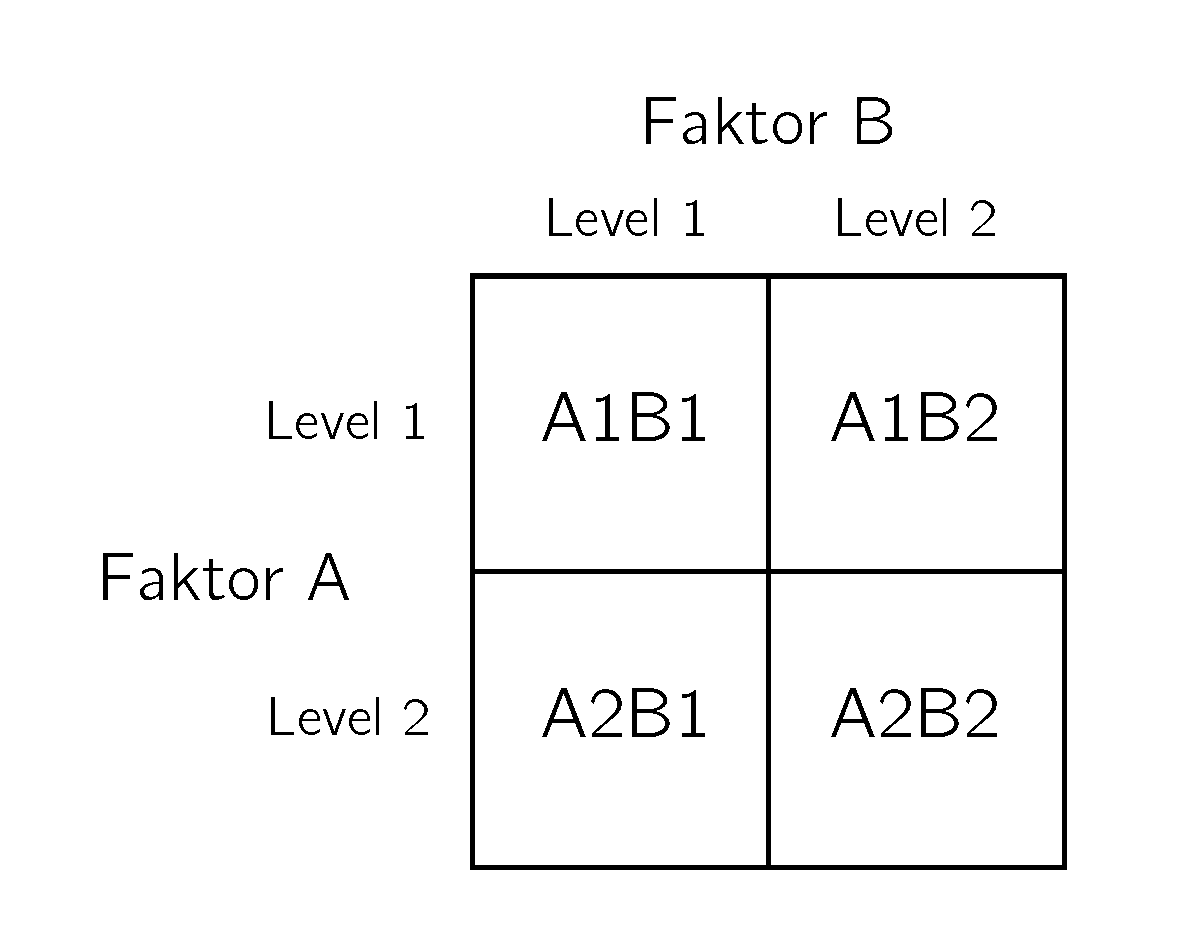
\includegraphics[width=0.65\linewidth]{11_Abbildungen/alm_11_zva_konzept} \end{center}

\center
\small

Die Zellen/Gruppen des Designs sind hier mit A1B1, A1B2, A2B1 und A2B2
bezeichnet.
\end{frame}

\begin{frame}{Anwendungsszenario}
\protect\hypertarget{anwendungsszenario-2}{}
\vspace{2mm}

\textcolor{darkblue}{Datennotation}

\begin{center}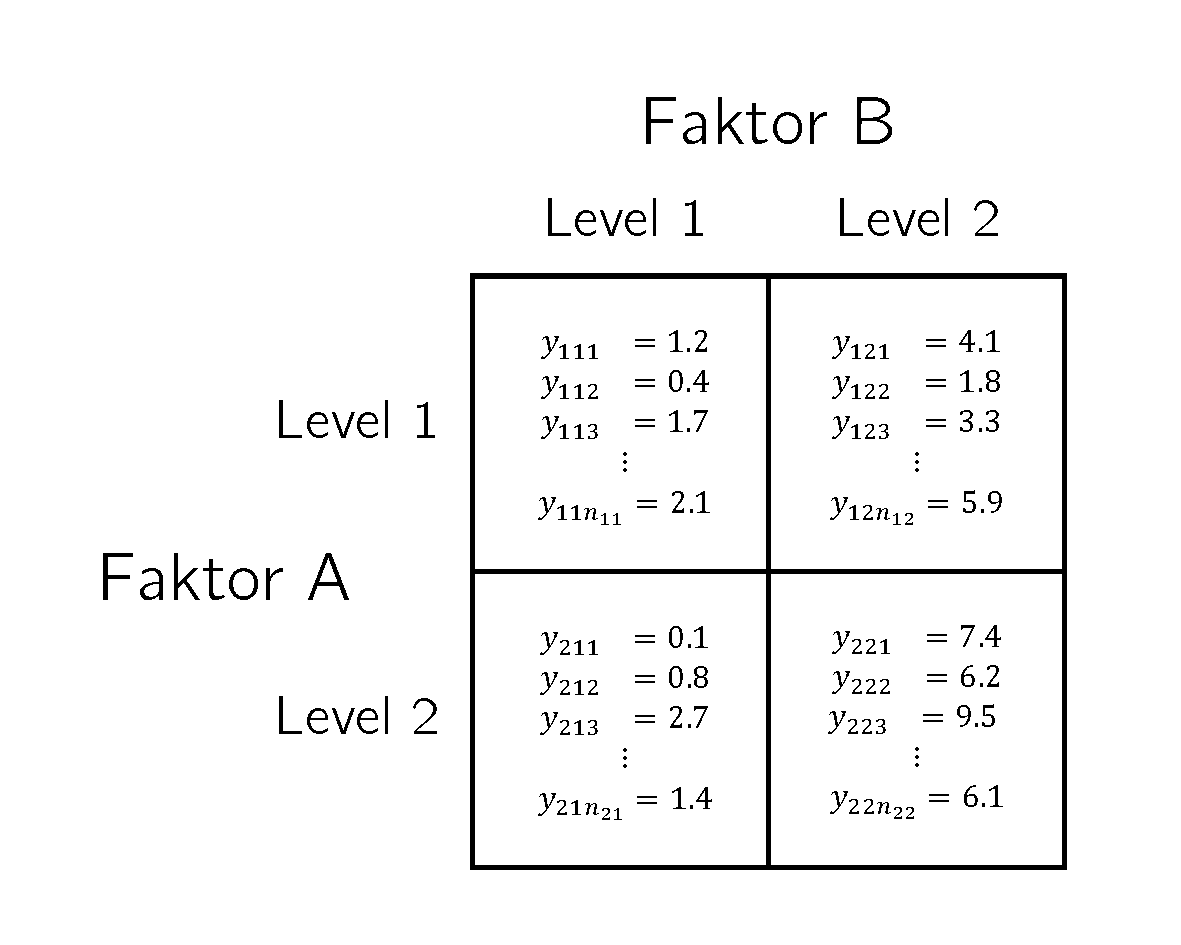
\includegraphics[width=0.7\linewidth]{11_Abbildungen/alm_11_zva_datennotation} \end{center}

\center
\small

\(y_{ijk}\) bezeichnet die Datenvariable der \(k\)ten experimentellen
Einheit (\(k = 1,...,n_{ij}\)) im \(i\)ten Level von Faktor A und
\(j\)ten Level von Faktor B (\(i = 1,2, j = 1,2\))
\end{frame}

\begin{frame}{Anwendungsszenario}
\protect\hypertarget{anwendungsszenario-3}{}
\textcolor{darkblue}{Datentabellenform mit $n_{ij} := 12, 1 \le i,j \le 2$}

\small
\center

\begin{longtable}[]{@{}lrrrr@{}}
\toprule
& \(y_{11k}\) & \(y_{12k}\) & \(y_{21k}\) & \(y_{22k}\) \\
\midrule
\endhead
1 & 2.37 & 4.38 & 4.12 & 6.61 \\
2 & 3.18 & 2.79 & 3.44 & 6.94 \\
3 & 2.16 & 6.12 & 3.34 & 8.10 \\
4 & 4.59 & 4.96 & 2.03 & 7.76 \\
5 & 3.33 & 4.98 & 3.02 & 6.83 \\
6 & 2.18 & 5.94 & 3.92 & 6.75 \\
7 & 3.49 & 5.82 & 4.86 & 7.70 \\
8 & 3.74 & 5.59 & 3.40 & 7.56 \\
9 & 3.58 & 5.92 & 3.89 & 6.31 \\
10 & 2.69 & 5.78 & 3.45 & 6.29 \\
11 & 4.51 & 5.08 & 2.12 & 7.37 \\
12 & 3.39 & 3.01 & 3.08 & 7.77 \\
\bottomrule
\end{longtable}

\vspace{-2mm}
\center
\small

\(y_{ijk}\) bezeichnet die Datenvariable der \(k\)ten experimentellen
Einheit (\(k = 1,...,n_{ij}\)) im \(i\)ten Level von Faktor A und
\(j\)ten Level von Faktor B (\(i = 1,2, j = 1,2\))
\end{frame}

\begin{frame}{Anwendungsszenario}
\protect\hypertarget{anwendungsszenario-4}{}
\textcolor{darkblue}{Datendeskription durch Boxplot}

\vspace{3mm}
\center

\begin{center}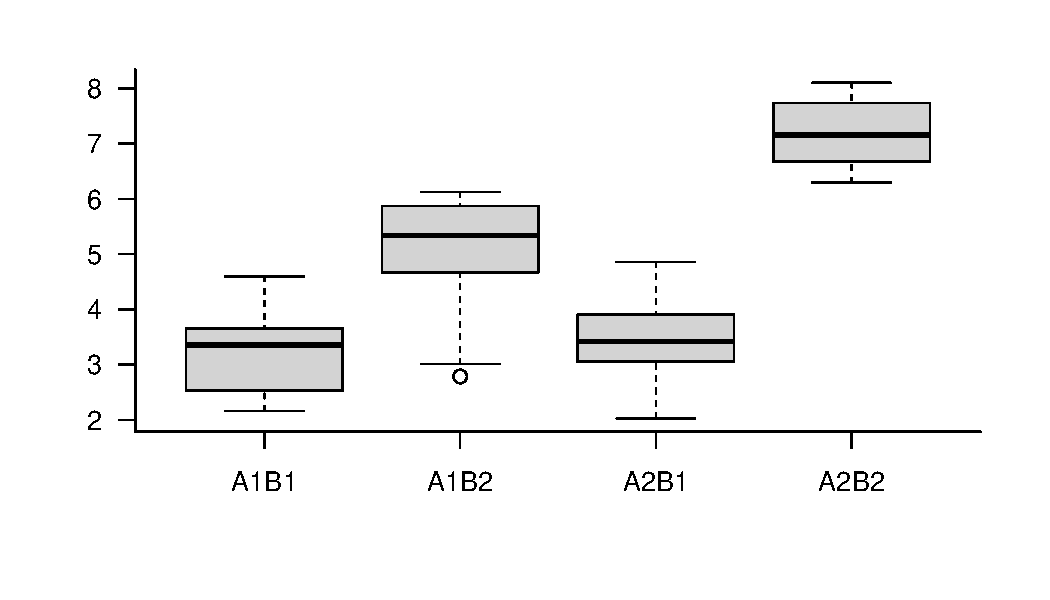
\includegraphics[width=0.95\linewidth]{11_Abbildungen/alm_11_zva_boxplot} \end{center}
\end{frame}

\begin{frame}{Anwendungsszenario}
\protect\hypertarget{anwendungsszenario-5}{}
\textcolor{darkblue}{Haupteffekte (main effects) und Interaktionen (interactions)}
\small

Man unterscheidet intuitiv hinsichtlich der Gruppenmittelwerte
\emph{Haupteffekte} und \emph{Interaktionen}

\footnotesize

\begin{itemize}
\tightlist
\item
  \justifying Intuitiv spricht man vom Vorliegen eines
  \emph{Haupteffekts von Faktor A}, wenn sich die Gruppenmittelwerte
  zwischen Level 1 und Level 2 von Faktor A, jeweils gemittelt über die
  zwei Level von Faktor B, unterscheiden.
\item
  Intuitiv spricht man vom Vorliegen eines \emph{Haupteffekts von Faktor
  B}, wenn sich die Gruppenmittelwerte zwischen Level 1 und Level 2 von
  Faktor B, jeweils gemittelt über die zwei Level von Faktor A,
  unterscheiden.
\item
  Intuitiv spricht man vom Vorliegen einer \emph{Interaktion der
  Faktoren A und B}, wenn der Unterschied der Gruppenmittelwerte von
  Faktor A zwischen Level 1 und 2 unterschiedlich für Level 1 und Level
  2 von Faktor B ausgeprägt ist bzw. wenn der Unterschied der
  Gruppenmittelwerte von Faktor B zwischen Level 1 und 2 unterschiedlich
  für Level 1 und Level 2 von Faktor A ausgeprägt ist.
\end{itemize}

\small

Intuitiv beziehen sich Haupteffekte also auf (marginale) Unterschiede
(Differenzen), während sich Interaktionen auf Unterschiede von
Unterschieden (Differenzen von Differenzen) beziehen.

Das Vorhandensein einer Interaktion besagt lediglich, dass sich die
Unterschiede der Gruppenmittelwerte zwischen den Leveln eines
experimentellen Faktors in Abhängigkeit von den Leveln des anderen
experimentellen Faktors ändern, es macht aber keine Aussage darüber,
warum dies so ist.

\flushright

\(\Rightarrow\) Haupteffekte und Interaktionen sind Datenmuster, keine
wissenschaftlichen Theorien.
\end{frame}

\begin{frame}{Anwendungsszenario}
\protect\hypertarget{anwendungsszenario-6}{}
\vspace{1mm}

\textcolor{darkblue}{Datendeskription durch Barplot}

\vspace{3mm}
\center

\begin{center}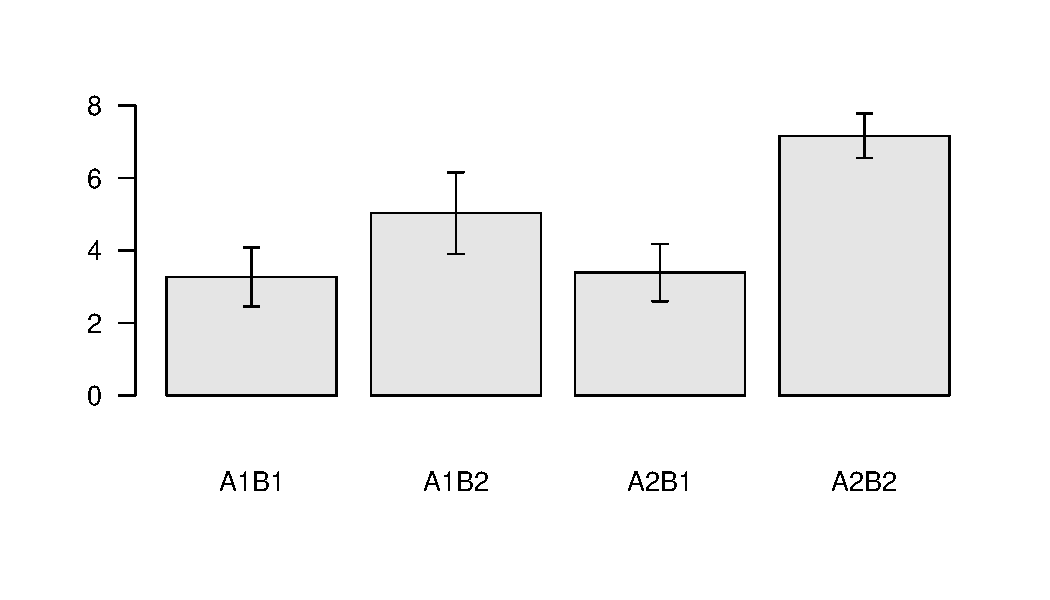
\includegraphics[width=0.95\linewidth]{11_Abbildungen/alm_11_zva_barplot} \end{center}
\end{frame}

\begin{frame}{Anwendungsszenario}
\protect\hypertarget{anwendungsszenario-7}{}
\vspace{2mm}

\textcolor{darkblue}{Datendeskription durch Lineplot}

\vspace{3mm}
\center

\begin{center}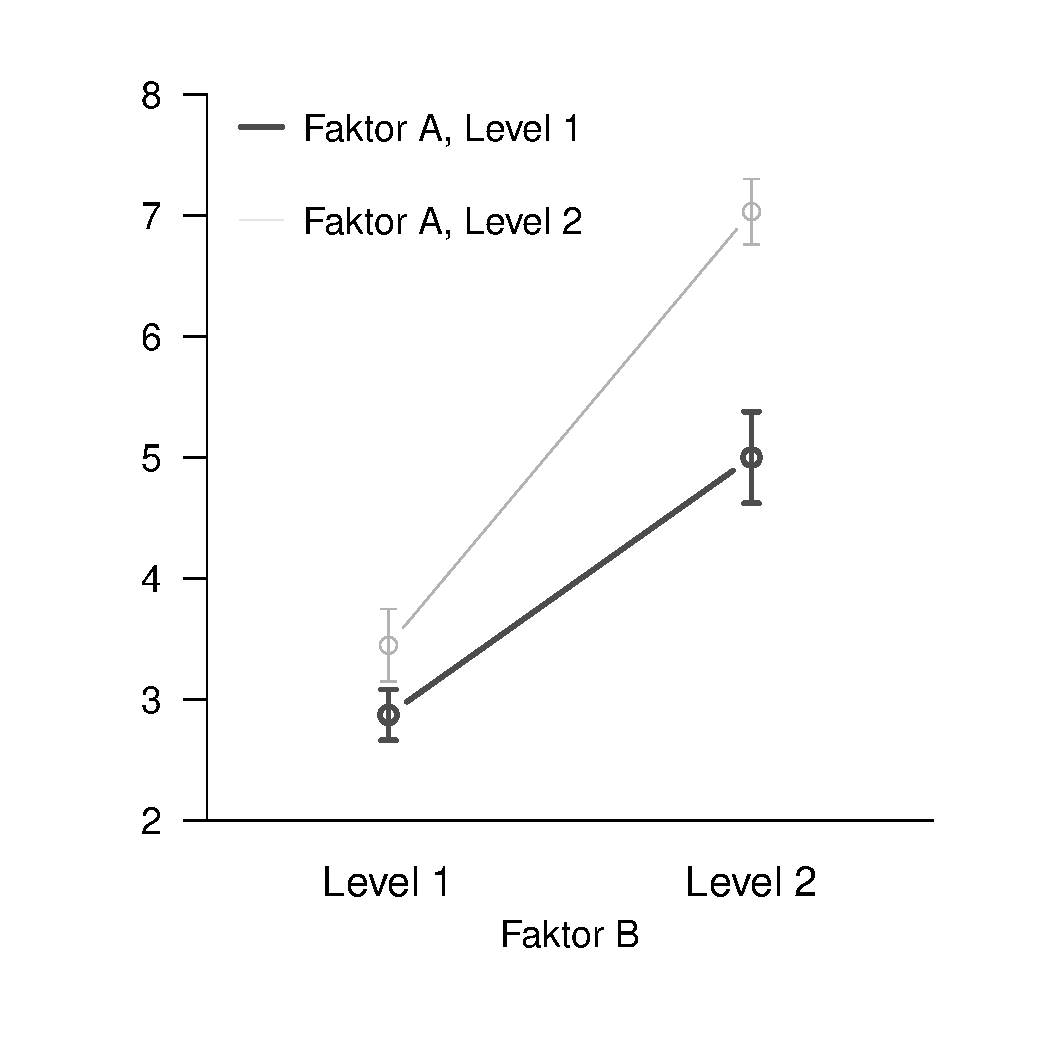
\includegraphics[width=0.65\linewidth]{11_Abbildungen/alm_11_zva_lineplot} \end{center}
\end{frame}

\begin{frame}{Anwendungsszenario}
\protect\hypertarget{anwendungsszenario-8}{}
\setstretch{1.6}

\textcolor{darkblue}{Anwendungsbeispiel}

BDI Datenanalyse bei zwei Therapiearten für zwei Altersklassen

\small

\begin{itemize}
\tightlist
\item
  Faktor (A) Therapie mit Level (1) Face-to-face (F2F) und Level (2)
  Online (ONL)
\item
  Faktor (B) Altersklasse mit Level (1) Young Adults (YA) und (2) und
  Older Adults (OA)
\item
  \(n_{ij} := 20, 1 \le i,j \le 2\) Patient:innen in jeder Bedingung,
  \(n = 80\) Patient:innen insgesamt.
\end{itemize}

\normalsize

2 x 2 randomisiertes zweifaktorielles Studiendesigns \(\Rightarrow\) 2 x
2 ANOVA

\begin{itemize}
\tightlist
\item
  Inferentielle Evidenz für einen Haupteffekt der Therapieart?
\item
  Inferentielle Evidenz für einen Haupteffekt der Altersklasse?
\item
  Inferentielle Evidenz für Interaktion (Verschiedene Therapieeffekte
  zwischen Altersklassen)?
\end{itemize}
\end{frame}

\begin{frame}[fragile]{Anwendungsszenario}
\protect\hypertarget{anwendungsszenario-9}{}
\textcolor{darkblue}{Anwendungsbeispiel} \vspace{1mm} \setstretch{1}
\tiny

\begin{Shaded}
\begin{Highlighting}[]
\NormalTok{fname       }\OtherTok{=} \FunctionTok{file.path}\NormalTok{(}\FunctionTok{getwd}\NormalTok{(), }\StringTok{"11\_Daten"}\NormalTok{, }\StringTok{"11\_Zweifaktorielle\_Varianzanalyse\_Daten.csv"}\NormalTok{)}
\NormalTok{D           }\OtherTok{=} \FunctionTok{read.table}\NormalTok{(fname, }\AttributeTok{sep =} \StringTok{","}\NormalTok{, }\AttributeTok{header =} \ConstantTok{TRUE}\NormalTok{)}
\end{Highlighting}
\end{Shaded}

\begin{longtable}[]{@{}lcccc@{}}
\toprule
& ID & Therapy & Age & BDI \\
\midrule
\endhead
1 & 1 & F2F & YA & 5.82 \\
2 & 2 & F2F & YA & 7.15 \\
3 & 3 & F2F & YA & 7.00 \\
4 & 4 & F2F & YA & 6.11 \\
5 & 5 & F2F & YA & 7.58 \\
6 & 6 & F2F & YA & 4.49 \\
21 & 21 & F2F & OA & 6.73 \\
22 & 22 & F2F & OA & 8.14 \\
23 & 23 & F2F & OA & 4.91 \\
24 & 24 & F2F & OA & 6.27 \\
25 & 25 & F2F & OA & 10.96 \\
26 & 26 & F2F & OA & 9.87 \\
41 & 41 & ONL & YA & 5.53 \\
42 & 42 & ONL & YA & 6.20 \\
43 & 43 & ONL & YA & 3.88 \\
44 & 44 & ONL & YA & 3.21 \\
45 & 45 & ONL & YA & 3.17 \\
46 & 46 & ONL & YA & 1.25 \\
61 & 61 & ONL & OA & 3.19 \\
62 & 62 & ONL & OA & 3.64 \\
63 & 63 & ONL & OA & 3.89 \\
64 & 64 & ONL & OA & 1.97 \\
65 & 65 & ONL & OA & 1.91 \\
66 & 66 & ONL & OA & 4.25 \\
\bottomrule
\end{longtable}
\end{frame}

\begin{frame}[fragile]{Anwendungsszenario}
\protect\hypertarget{anwendungsszenario-10}{}
\textcolor{darkblue}{Anwendungsbeispiel} \vspace{1mm} \tiny
\setstretch{.9}

\begin{Shaded}
\begin{Highlighting}[]
\CommentTok{\# Datenreformatierung}
\NormalTok{fname  }\OtherTok{=} \FunctionTok{file.path}\NormalTok{(}\FunctionTok{getwd}\NormalTok{(), }\StringTok{"11\_Daten"}\NormalTok{, }\StringTok{"11\_Zweifaktorielle\_Varianzanalyse\_Daten.csv"}\NormalTok{)}
\NormalTok{D      }\OtherTok{=} \FunctionTok{read.table}\NormalTok{(fname, }\AttributeTok{sep =} \StringTok{","}\NormalTok{, }\AttributeTok{header =} \ConstantTok{TRUE}\NormalTok{)}
\NormalTok{A1B1   }\OtherTok{=}\NormalTok{ D}\SpecialCharTok{$}\NormalTok{BDI[D}\SpecialCharTok{$}\NormalTok{Therapy }\SpecialCharTok{==} \StringTok{"F2F"} \SpecialCharTok{\&}\NormalTok{ D}\SpecialCharTok{$}\NormalTok{Age }\SpecialCharTok{==} \StringTok{"YA"}\NormalTok{ ]}
\NormalTok{A1B2   }\OtherTok{=}\NormalTok{ D}\SpecialCharTok{$}\NormalTok{BDI[D}\SpecialCharTok{$}\NormalTok{Therapy }\SpecialCharTok{==} \StringTok{"F2F"} \SpecialCharTok{\&}\NormalTok{ D}\SpecialCharTok{$}\NormalTok{Age }\SpecialCharTok{==} \StringTok{"OA"}\NormalTok{ ]}
\NormalTok{A2B1   }\OtherTok{=}\NormalTok{ D}\SpecialCharTok{$}\NormalTok{BDI[D}\SpecialCharTok{$}\NormalTok{Therapy }\SpecialCharTok{==} \StringTok{"ONL"} \SpecialCharTok{\&}\NormalTok{ D}\SpecialCharTok{$}\NormalTok{Age }\SpecialCharTok{==} \StringTok{"YA"}\NormalTok{ ]}
\NormalTok{A2B2   }\OtherTok{=}\NormalTok{ D}\SpecialCharTok{$}\NormalTok{BDI[D}\SpecialCharTok{$}\NormalTok{Therapy }\SpecialCharTok{==} \StringTok{"ONL"} \SpecialCharTok{\&}\NormalTok{ D}\SpecialCharTok{$}\NormalTok{Age }\SpecialCharTok{==} \StringTok{"OA"}\NormalTok{ ]}
\NormalTok{Y      }\OtherTok{=} \FunctionTok{data.frame}\NormalTok{(}\StringTok{"F2F YA"} \OtherTok{=}\NormalTok{ A1B1, }\StringTok{"F2F OA"} \OtherTok{=}\NormalTok{ A1B2, }\StringTok{"ONL YA"} \OtherTok{=}\NormalTok{ A2B1, }\StringTok{"ONL OA"} \OtherTok{=}\NormalTok{ A2B2)}
\end{Highlighting}
\end{Shaded}

\begin{longtable}[]{@{}lrrrr@{}}
\toprule
& F2F.YA & F2F.OA & ONL.YA & ONL.OA \\
\midrule
\endhead
1 & 5.82 & 6.73 & 5.526 & 3.188 \\
2 & 7.15 & 8.14 & 6.200 & 3.642 \\
3 & 7.00 & 4.91 & 3.881 & 3.888 \\
4 & 6.11 & 6.27 & 3.211 & 1.968 \\
5 & 7.58 & 10.96 & 3.170 & 1.910 \\
6 & 4.49 & 9.87 & 1.246 & 4.250 \\
7 & 5.13 & 4.74 & 3.892 & -2.429 \\
8 & 8.22 & 7.68 & 4.775 & 0.758 \\
9 & 5.58 & 5.78 & 3.794 & 2.780 \\
10 & 7.95 & 7.80 & 6.717 & 5.024 \\
11 & 11.35 & 8.76 & 4.836 & 1.389 \\
12 & 7.31 & 6.78 & 3.044 & 3.152 \\
13 & 9.93 & 8.54 & 1.058 & 3.477 \\
14 & 3.39 & 7.73 & 3.688 & 2.975 \\
15 & 7.38 & 5.58 & 3.888 & 0.359 \\
16 & 5.51 & 5.62 & 5.240 & 2.659 \\
17 & 7.06 & 8.11 & 0.021 & 5.191 \\
18 & 8.38 & 8.39 & 4.149 & 0.329 \\
19 & 6.92 & 6.49 & 5.564 & 2.367 \\
20 & 11.80 & 6.67 & 5.838 & 0.747 \\
\bottomrule
\end{longtable}
\end{frame}

\begin{frame}{Anwendungsszenario}
\protect\hypertarget{anwendungsszenario-11}{}
\vspace{1mm}

\textcolor{darkblue}{Datendeskription durch Barplot}

\vspace{3mm}
\center

\begin{center}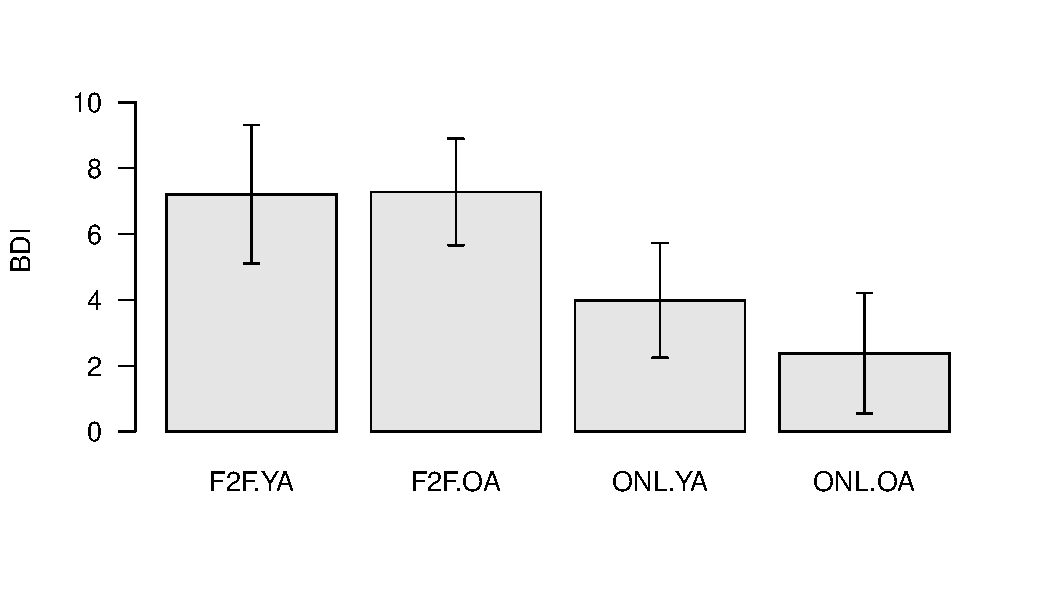
\includegraphics[width=0.95\linewidth]{11_Abbildungen/alm_11_zva_barplot_beispiel} \end{center}
\end{frame}

\begin{frame}{Anwendungsszenario}
\protect\hypertarget{anwendungsszenario-12}{}
\vspace{2mm}

\textcolor{darkblue}{Datendeskription durch Lineplot}

\vspace{3mm}
\center

\begin{center}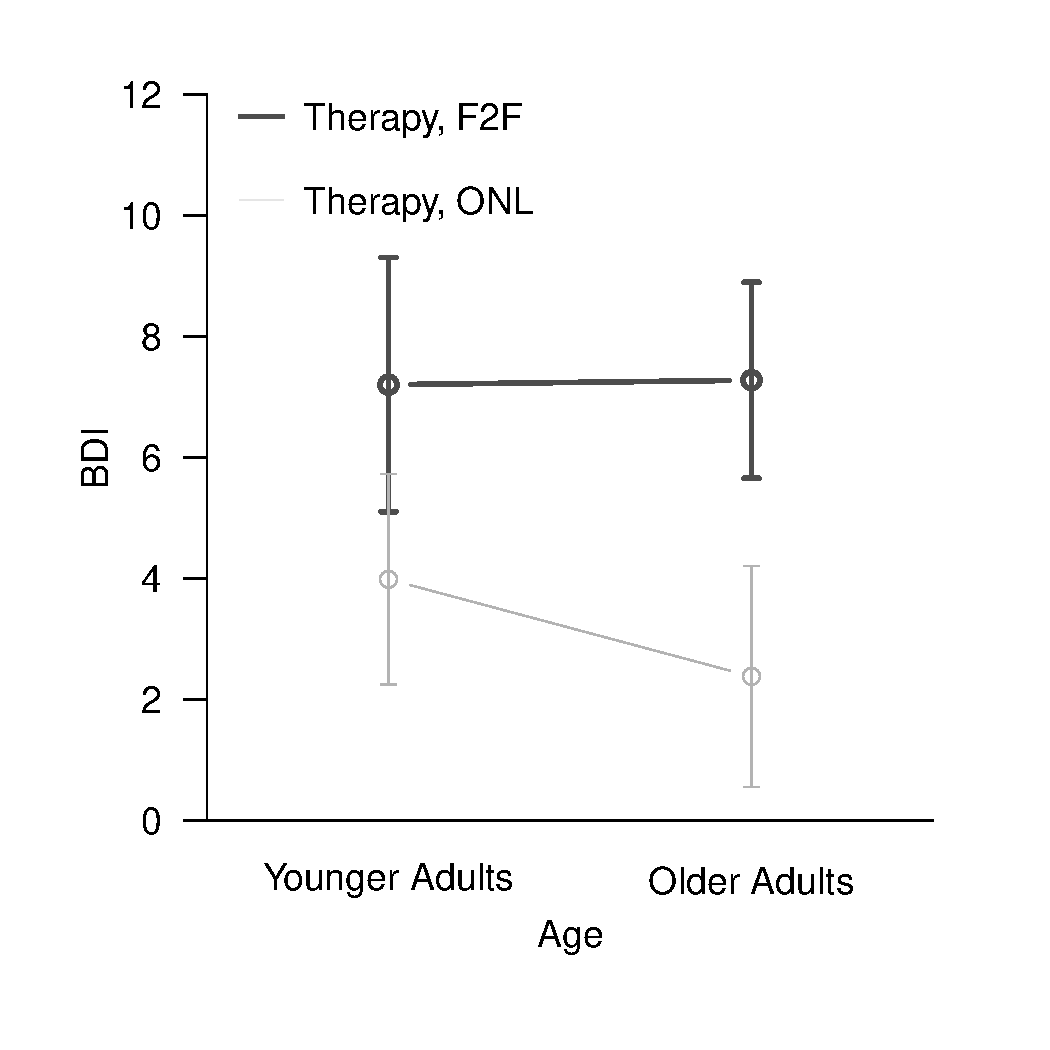
\includegraphics[width=0.6\linewidth]{11_Abbildungen/alm_11_zva_lineplot_beispiel} \end{center}
\end{frame}

\begin{frame}{}
\protect\hypertarget{section-5}{}
\large
\setstretch{2.7}
\vfill

Anwendungsszenario

\textbf{Modellformulierung}

Modellschätzung

Modellevaluation

Selbstkontrollfragen \vfill
\end{frame}

\begin{frame}{Modellformulierung}
\protect\hypertarget{modellformulierung}{}
\vspace{1mm}

\textcolor{darkblue}{Modell der additiven ZVA} \setstretch{1.2}
\footnotesize

In Analogie zur einfaktoriellen Varianzanalyse (EVA) möchte man in der
additiven ZVA die Gruppenerwartungswerte \(\mu_{ij}\) mit
\(i = 1,...,I\) für die Level von Faktor A und \(j = 1,...,J\) für die
Level von Faktor B als Summe eines gruppenunspezifischen
Erwartungswertes und den Effekten der Level von Faktor A und der Level
von Faktor B modellieren.

Wir bezeichnen den gruppenunspezifischen Erwartungswertparameter mit
\(\mu_0\), den Effekt von Level \(i\) von Faktor A mit \(\alpha_i\) und
den Effekt von Level \(j\) von Faktor B mit \(\beta_j\) (\(\beta_j\)
bezeichnet hier also \underline{nicht} den \(j\)ten Eintrag des
Betaparametervektors). Dann ergibt sich zum Beispiel für \(I := J := 2\)

\begin{center}
\begin{tabular}{l|l}
$\mu_{11} := \mu_0 + \alpha_1 + \beta_1$ & $\mu_{12} := \mu_0 + \alpha_1 + \beta_2$ \\\hline
$\mu_{21} := \mu_0 + \alpha_2 + \beta_1$ & $\mu_{22} := \mu_0 + \alpha_2 + \beta_2$ \\
\end{tabular}
\end{center}

Wie im Falle der EVA ist diese Darstellung der Gruppenerwartungswerte
\(\mu_{ij}\) allerdings überparameterisiert. Um eine eindeutige
Darstellung der \(\mu_{ij}\) zu gewährleisten, bietet sich auch hier die
Restriktion an, den Effekt des ersten Levels jedes Faktors als Null zu
definieren \begin{equation}
\alpha_1 := \beta_1 := 0.
\end{equation} und damit die Faktorlevelkombination A1B1 als
Referenzgruppe zu etablieren. Es ergibt sich somit zum Beispiel für für
\(I := J := 2\)

\begin{center}
\begin{tabular}{l|l}
$\mu_{11} := \mu_0$            & $\mu_{12} := \mu_0 + \beta_2$            \\\hline
$\mu_{21} := \mu_0 + \alpha_2$ & $\mu_{22} := \mu_0 + \alpha_2 + \beta_2$ \\
\end{tabular}
\end{center}

Auch bei dieser Effektdarstellung des Modells der additiven 2 x 2 ZVA
mit Referenzgruppe ändern sich die Interpretation der Parameter
\(\mu_0,\alpha_2,\beta_2\) im Vergleich zum überparameterisierten Fall
ohne Referenzgruppe: \(\mu_0\) entspricht dem Erwartungswert der
Faktorlevelkombination A1B1, \(\alpha_2\) der Differenz beim Übergang
von Level 1 zu Level 2 von Faktor A und \(\beta_2\) der Differenz beim
Übergang von Level 1 zu Level 2 von Faktor B.
\end{frame}

\begin{frame}{Modellformulierung}
\protect\hypertarget{modellformulierung-1}{}
\footnotesize
\begin{definition}[Modell der additiven ZVA mit Referenzgruppe]
\justifying
$y_{ijk}$ mit $i = 1,...,I, j = 1,...,J, k = 1,...,n_{ij}$ sei die Zufallsvariable,
die den $k$ten Datenpunkt zum $i$ten Level von Faktor A und dem $j$ten Level von
Faktor B in einem ZVA Anwendungsszenario modelliert. Dann hat das
\textit{Modell der additiven ZVA mit Referenzgruppe} die strukturelle Form
\begin{equation}
y_{ijk} = \mu_{ij} + \varepsilon_{ijk} \sim N(0,\sigma^2)
\mbox{ u.i.v. für } i = 1,...,I, j = 1,...,J, k = 1,...,n_{ij}
\end{equation}
und die Datenverteilungsform
\begin{equation}
y_{ijk} \sim N(\mu_{ij}, \sigma^2) \mbox{ u.i.v. für } i = 1,...,I, j = 1,...,J, k = 1,...,n_{ij}
\end{equation}
mit
\begin{equation}
\mu_{ij} := \mu_0 + \alpha_i + \beta_j \mbox{ für } i = 1,...,I, j = 1,...,J \mbox{ mit } \alpha_1 := \beta_1 := 0.
\end{equation}
und $\sigma^2 > 0$.
\end{definition}

Bemerkungen

\begin{itemize}
\tightlist
\item
  Das Modell der additiven ZVA modelliert ausschließlich Haupteffekte,
  keine Interaktionen.
\item
  Wir verzichten auf die Angabe einer allgemeinen Designmatrixform
  dieses Modells.
\end{itemize}
\end{frame}

\begin{frame}{Modellformulierung}
\protect\hypertarget{modellformulierung-2}{}
\textcolor{darkblue}{Parameterbeispiele}

\small
\setstretch{1.5}

\noindent (1) Es sei \(\mu_0 := 1, \alpha_2 := 1, \beta_2 := 0\). Dann
gilt:

\begin{center}
\begin{tabular}{ll}
$\bm{\mu_{11}} = \mu_0 + \alpha_1 + \beta_1 = 1 + 0 + 0 = \bm{1}$
&
$\bm{\mu_{12}} = \mu_0 + \alpha_1 + \beta_2 = 1 + 0 + 0 = \bm{1}$
\\
$\bm{\mu_{21}} = \mu_0 + \alpha_2 + \beta_1 = 1 + 1 + 0 = \bm{2}$
&
$\bm{\mu_{22}} = \mu_0 + \alpha_2 + \beta_2 = 1 + 1 + 0 = \bm{2}$ \\
\end{tabular}
\end{center}

\(\Rightarrow\) Haupteffekt von Faktor A, kein Haupteffekt von Faktor B
\vspace{1mm}

\noindent (2) Es sei \(\mu_0 := 1, \alpha_2 := 0, \beta_2 := 1\). Dann
gilt:

\begin{center}
\begin{tabular}{ll}
$\bm{\mu_{11}} = \mu_0 + \alpha_1 + \beta_1 = 1 + 0 + 0 = \bm{1}$
&
$\bm{\mu_{12}} = \mu_0 + \alpha_1 + \beta_2 = 1 + 0 + 1 = \bm{2}$
\\
$\bm{\mu_{21}} = \mu_0 + \alpha_2 + \beta_1 = 1 + 0 + 0 = \bm{1}$
&
$\bm{\mu_{22}} = \mu_0 + \alpha_2 + \beta_2 = 1 + 0 + 1 = \bm{2}$ \\
\end{tabular}
\end{center}

\(\Rightarrow\) Kein Haupteffekt von Faktor A, Haupteffekt von Faktor B
\vspace{1mm}

\noindent (3) Es sei \(\mu_0 := 1, \alpha_2 := 1, \beta_2 := 1\). Dann
gilt:

\begin{center}
\begin{tabular}{ll}
$\bm{\mu_{11}} = \mu_0 + \alpha_1 + \beta_1 = 1 + 0 + 0 = \bm{1}$
&
$\bm{\mu_{12}} = \mu_0 + \alpha_1 + \beta_2 = 1 + 0 + 1 = \bm{2}$
\\
$\bm{\mu_{21}} = \mu_0 + \alpha_2 + \beta_1 = 1 + 1 + 0 = \bm{2}$
&
$\bm{\mu_{22}} = \mu_0 + \alpha_2 + \beta_2 = 1 + 1 + 1 = \bm{3}$ \\
\end{tabular}
\end{center}

\(\Rightarrow\) Haupteffekt von Faktor A, Haupteffekt von Faktor B
\end{frame}

\begin{frame}{Modellformulierung}
\protect\hypertarget{modellformulierung-3}{}
\vspace{1mm}

\textcolor{darkblue}{Parameterbeispiele}

\vfill
\vspace{3mm}
\center

\begin{center}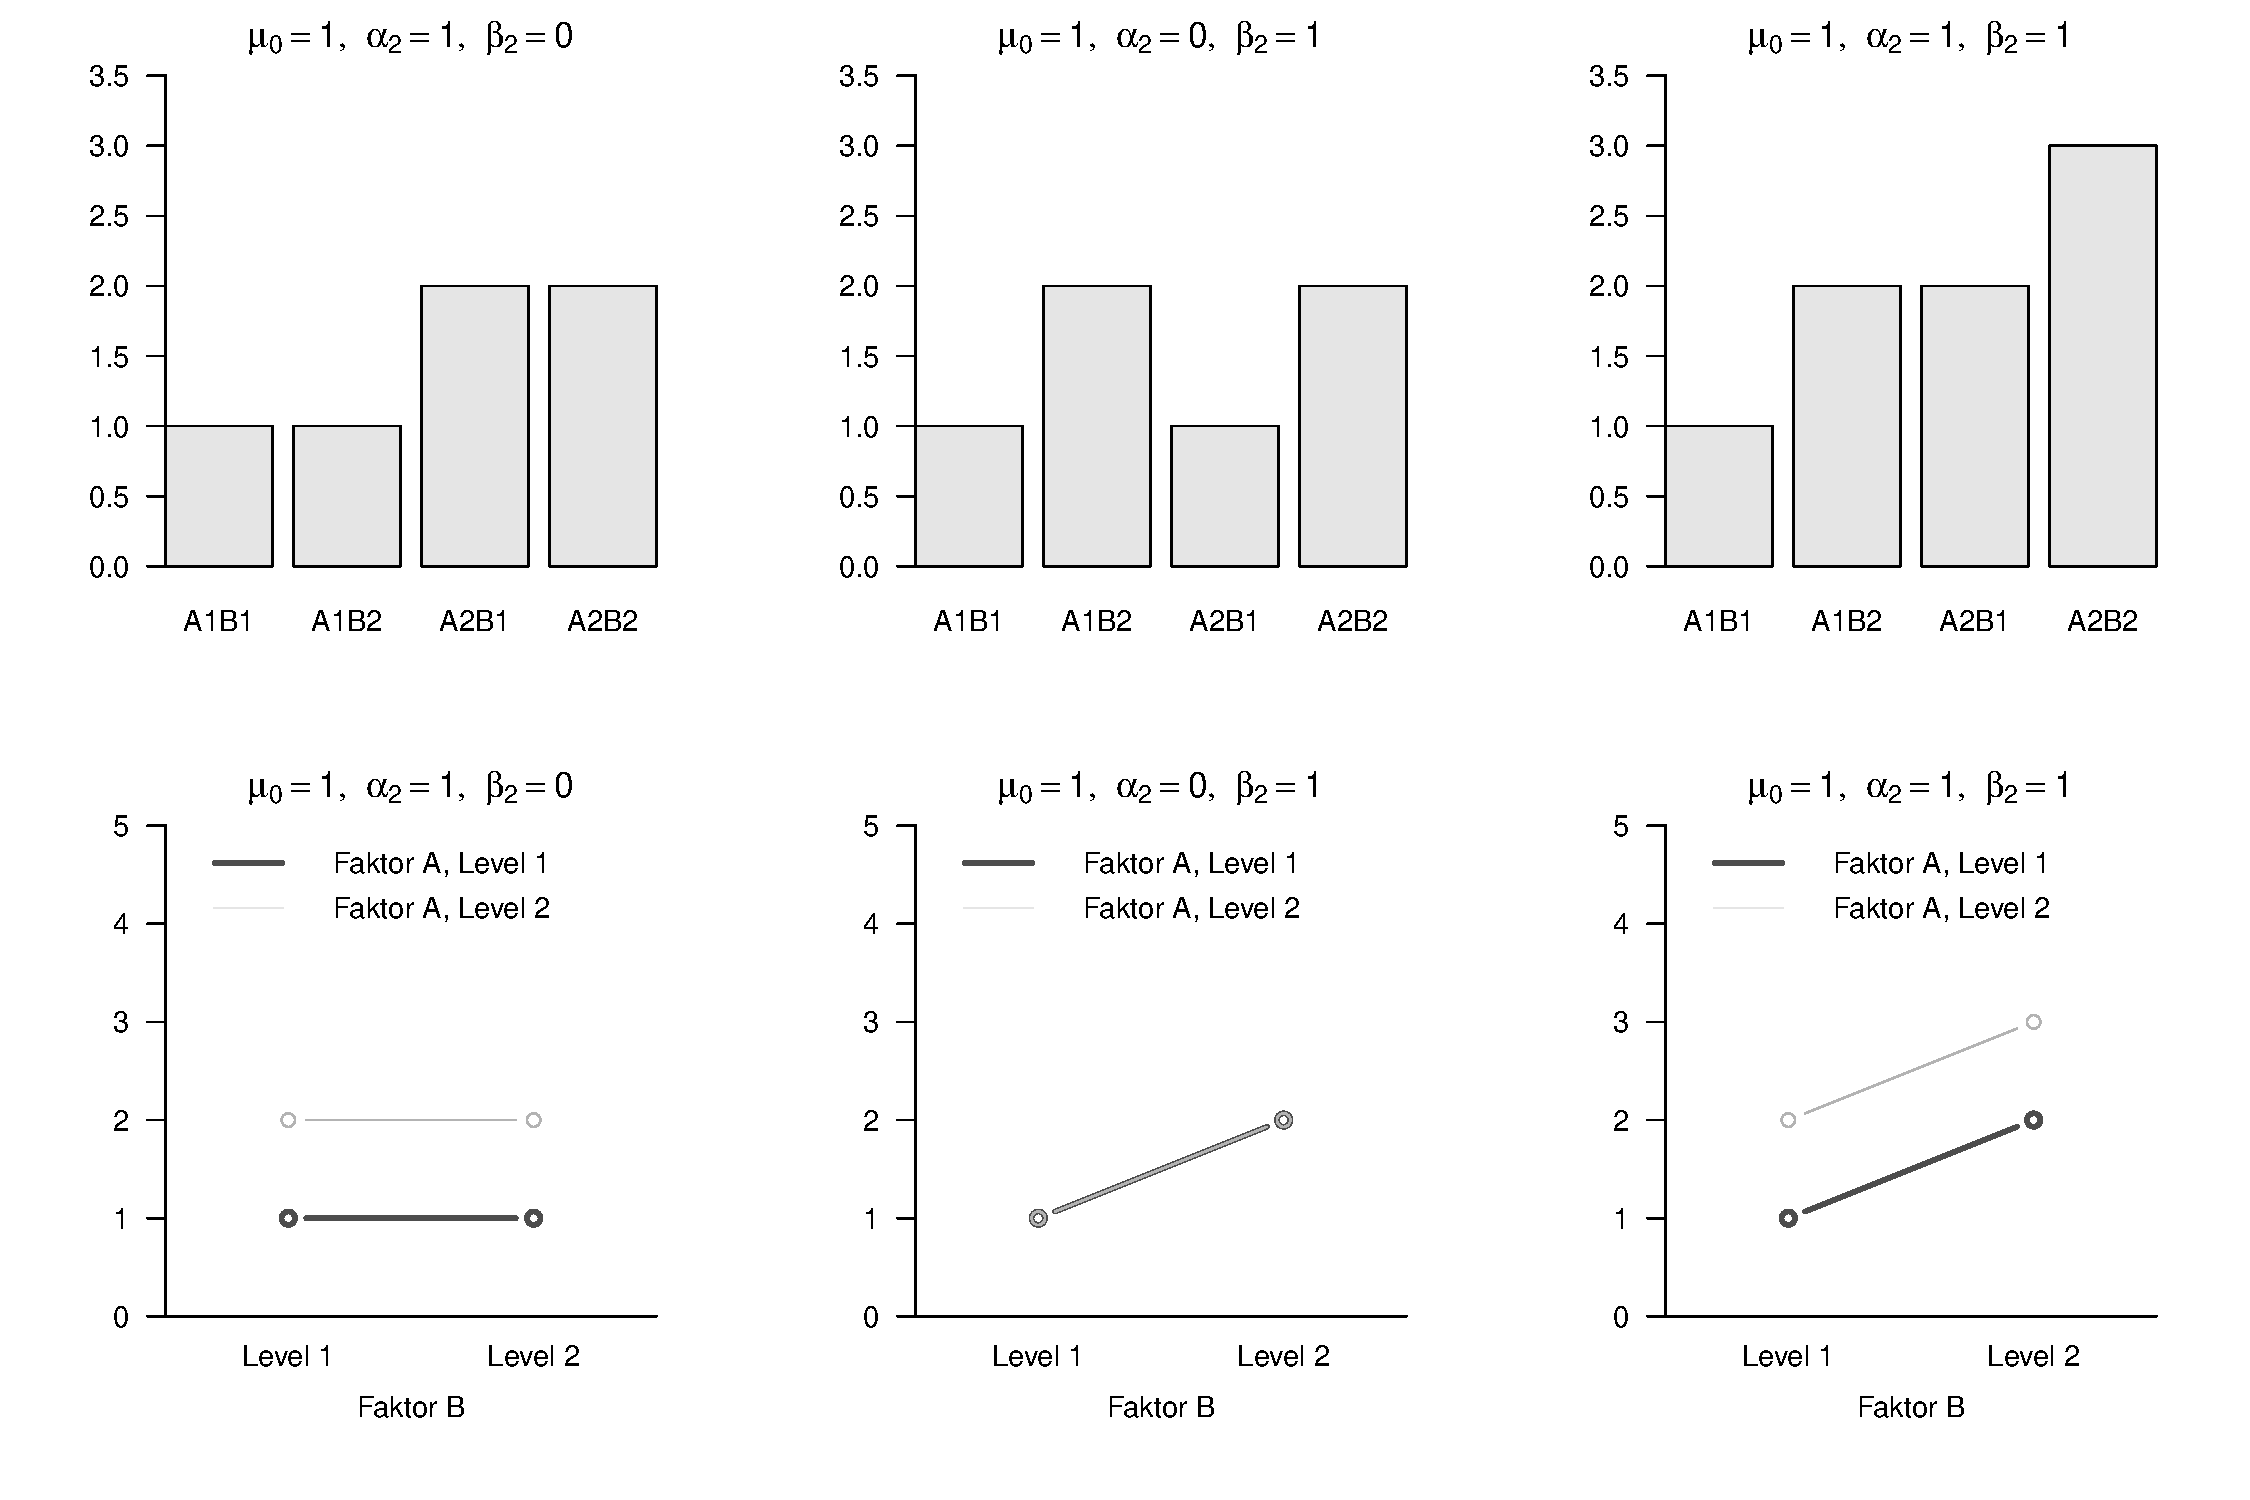
\includegraphics[width=1\linewidth]{11_Abbildungen/alm_11_zva_add_beispiel} \end{center}
\vfill
\end{frame}

\begin{frame}{Modellformulierung}
\protect\hypertarget{modellformulierung-4}{}
\footnotesize
\setstretch{1.2}
\vspace{2mm}
\begin{theorem}[Designmatrixform des Modells der 2 x 2 ZVA mit Referenzgruppe]
\justifying
\normalfont
Gegeben sei die strukturelle Form des Modells der 2 x 2 ZVA mit Referenzgruppe. 
Dann hat dieses Modell die Designmatrixform
\begin{equation}
y \sim N(X\beta,\sigma^2I_n),
\end{equation}
wobei
\begin{equation}
y:=
\begin{pmatrix}
y_{111}\\
\vdots \\
y_{11n_{11}}\\
y_{121}\\
\vdots \\
y_{12n_{12}}\\
y_{211}\\
\vdots \\
y_{21n_{21}}\\
y_{221}\\
\vdots \\
y_{22n_{22}}\\
\end{pmatrix}, \,
X =
\begin{pmatrix}
1       &   0       &   0           \\
\vdots  &   \vdots  &   \vdots      \\
1       &   0       &   0           \\
1       &   0       &   1           \\
\vdots  &   \vdots  &   \vdots      \\
1       &   0       &   1           \\
1       &   1       &   0           \\
\vdots  &   \vdots  &   \vdots      \\
1       &   1       &   0           \\
1       &   1       &   1           \\
\vdots  &   \vdots  &   \vdots      \\
1       &   1       &   1           \\
\end{pmatrix} \in \mathbb{R}^{n \times 3}, \,
\beta :=
\begin{pmatrix}
\mu_0               \\
\alpha_{2}          \\
\beta_{2}           \\
\end{pmatrix}
\in \mathbb{R}^{3}
\mbox{ und }
\sigma^2 > 0.
\end{equation}
\end{theorem}
\vspace{-2mm}

Bemerkung \vspace{-1mm}

\begin{itemize}
\tightlist
\item
  Das Theorem folgt direkt aus den Regel der Matrixmultiplikation.
\end{itemize}
\end{frame}

\begin{frame}{Modellformulierung}
\protect\hypertarget{modellformulierung-5}{}
\textcolor{darkblue}{Modell der ZVA mit Interaktion} \footnotesize
\setstretch{1.1}

In der ZVA mit Interaktion möchte man die Gruppenerwartungswerte
\(\mu_{ij}\) mit \(i = 1,...,I\) für die Level von Faktor A und
\(j = 1,...,J\) für die Level von Faktor B als Summe eines
gruppenunspezifischen Erwartungswertes, der Effekte der Level von Faktor
A und Faktor B und der Interaktion der Level der Faktoren modellieren.

Wir bezeichnen den gruppenunspezifischen Erwartungswertparameter mit
\(\mu_0\), den Effekt von Level \(i\) von Faktor A mit \(\alpha_i\), den
Effekt von Level \(j\) von Faktor B mit \(\beta_j\), und die Interaktion
von Level \(i\) von Faktor A mit Level \(j\) von Faktor B mit
\(\gamma_{ij}\). Dann ergibt sich zum Beispiel für \(I := J := 2\)

\begin{center}
\begin{tabular}{l|l}
$\mu_{11} := \mu_0 + \alpha_1 + \beta_1 + \gamma_{11}$ & $\mu_{12} := \mu_0 + \alpha_1 + \beta_2 + \gamma_{12}$ \\\hline
$\mu_{21} := \mu_0 + \alpha_2 + \beta_1 + \gamma_{21}$ & $\mu_{22} := \mu_0 + \alpha_2 + \beta_2 + \gamma_{22}$ \\
\end{tabular}
\end{center}

Wie in der die additiven ZVA ist diese Darstellung der
Gruppenerwartungswerte \(\mu_{ij}\) multipel überparameterisiert. Um
eine eindeutige Darstellung der \(\mu_{ij}\) zu gewährleisten, bietet
sich auch hier die Restriktion an, den Effekt des ersten Levels jedes
Faktors und jeder Interaktion als Null zu definieren \begin{equation}
\alpha_1 := \beta_1 := \gamma_{i1} := \gamma_{1j} := 0 \mbox{ für } i = 1,...,I, j = 1,..,J
\end{equation} und damit die Faktorlevelkombination A1B1 als
Referenzgruppe zu etablieren. Es ergibt sich somit zum Beispiel für für
\(I := J := 2\)

\begin{center}
\begin{tabular}{l|l}
$\mu_{11} := \mu_0$            & $\mu_{12} := \mu_0 + \beta_2$                          \\\hline
$\mu_{21} := \mu_0 + \alpha_2$ & $\mu_{22} := \mu_0 + \alpha_2 + \beta_2 + \gamma_{22}$ \\
\end{tabular}
\end{center}

Auch bei dieser Effektdarstellung des Modells der 2 x 2 ZVA mit
Interaktion und Referenzgruppe ändern sich die Interpretation der
Parameter \(\mu_0,\alpha_2,\beta_2,\gamma_{22}\) im Vergleich zum
überparameterisierten Fall ohne Referenzgruppe: \(\mu_0\) entspricht dem
Erwartungswert der Faktorlevelkombination A1B1, \(\alpha_2\) der
Differenz beim Übergang von Level 1 zu Level 2 von Faktor A, \(\beta_2\)
der Differenz beim Übergang von Level 1 zu Level 2 von Faktor B und
\(\gamma_{22}\) der Differenz beim Übergang von Level 1 zu Level 2 von
Faktor B im Unterschiede zum Übergang von Level 1 zu Level 2 von Faktor
A.
\end{frame}

\begin{frame}{Modellformulierung}
\protect\hypertarget{modellformulierung-6}{}
\footnotesize
\begin{definition}[Modell der ZVA mit Interaktion und Referenzgruppe]
\justifying
$y_{ijk}$ mit $i = 1,...,I, j = 1,...,J, k = 1,...,n_{ij}$ sei die Zufallsvariable,
die den $k$ten Datenpunkt zum $i$ten Level von Faktor A und dem $j$ten Level von
Faktor B in einem ZVA Anwendungsszenario modelliert. Dann hat das
\textit{Modell der ZVA mit Interaktion und Referenzgruppe} die strukturelle Form
\begin{equation}
y_{ijk} = \mu_{ij} + \varepsilon_{ijk} \sim N(0,\sigma^2)
\mbox{ u.i.v. für } i = 1,...,I, j = 1,...,J, k = 1,...,n_{ij}
\end{equation}
und die Datenverteilungsform
\begin{equation}
y_{ijk} \sim N(\mu_{ij}, \sigma^2) \mbox{ u.i.v. für } i = 1,...,I, j = 1,...,J, k = 1,...,n_{ij}
\end{equation}
mit
\begin{equation}
\mu_{ij} := \mu_0 + \alpha_i + \beta_j + \gamma_{ij}
\end{equation}
sowie
\begin{equation}
\alpha_1 := \beta_1 := \gamma_{i1} := \gamma_{1j} :=0 \mbox{ für } i = 1,...,I, j = 1,...,J
\end{equation}
und $\sigma^2 > 0$.
\end{definition}

Bemerkungen

\begin{itemize}
\tightlist
\item
  Wir verzichten auf die Angabe einer allgemeinen Designmatrixform
  dieses Modells.
\end{itemize}
\end{frame}

\begin{frame}{Modellformulierung}
\protect\hypertarget{modellformulierung-7}{}
\setstretch{1}

\textcolor{darkblue}{Parameterbeispiele}

\footnotesize

\noindent (1) Es sei
\(\mu_0 := 1, \alpha_2 := 0, \beta_2 := 0, \gamma_{22} = 2\). Dann gilt:

\begin{tiny}
\begin{tabular}{ll}
$\bm{\mu_{11}} = \mu_0 + \alpha_1 + \beta_1 + \gamma_{11} = 1 + 0 + 0 + 0=  \bm{1}$
&
$\bm{\mu_{12}} = \mu_0 + \alpha_1 + \beta_2 + \gamma_{12} = 1 + 0 + 0 + 0 = \bm{1}$
\\\\
$\bm{\mu_{21}} = \mu_0 + \alpha_2 + \beta_1 + \gamma_{21} = 1 + 0 + 0 + 0 = \bm{1}$
&
$\bm{\mu_{22}} = \mu_0 + \alpha_2 + \beta_2 + \gamma_{22} = 1 + 0 + 0 + 2 = \bm{3}$ \\
\end{tabular}
\end{tiny}
\vspace{2mm}
\footnotesize

\noindent (2) Es sei
\(\mu_0 := 1, \alpha_2 := 1, \beta_2 := 1, \gamma_{22} = -2\). Dann
gilt:

\begin{tiny}
\begin{tabular}{ll}
$\bm{\mu_{11}} = \mu_0 + \alpha_1 + \beta_1 + \gamma_{11} = 1 + 0 + 0 + 0=  \bm{1}$
&
$\bm{\mu_{12}} = \mu_0 + \alpha_1 + \beta_2 + \gamma_{12} = 1 + 0 + 1 + 0 = \bm{2}$
\\\\
$\bm{\mu_{21}} = \mu_0 + \alpha_2 + \beta_1 + \gamma_{21} = 1 + 0 + 1 + 0 = \bm{2}$
&
$\bm{\mu_{22}} = \mu_0 + \alpha_2 + \beta_2 + \gamma_{22} = 1 + 1 + 1 - 2 = \bm{1}$ \\
\end{tabular}
\end{tiny}
\vspace{2mm}

\noindent (3) Es sei
\(\mu_0 := 1, \alpha_2 := 1, \beta_2 := 0, \gamma_{22} = 1\). Dann gilt:

\begin{tiny}
\begin{tabular}{ll}
$\bm{\mu_{11}} = \mu_0 + \alpha_1 + \beta_1 + \gamma_{11} = 1 + 0 + 0 + 0 = \bm{1}$
&
$\bm{\mu_{12}} = \mu_0 + \alpha_1 + \beta_2 + \gamma_{12} = 1 + 0 + 0 + 0 = \bm{1}$
\\\\
$\bm{\mu_{21}} = \mu_0 + \alpha_2 + \beta_1 + \gamma_{21} = 1 + 1 + 0 + 0 = \bm{2}$
&
$\bm{\mu_{22}} = \mu_0 + \alpha_2 + \beta_2 + \gamma_{22} = 1 + 1 + 0 + 1 = \bm{3}$ \\
\end{tabular}
\end{tiny}
\vspace{2mm}

\noindent (4) Es sei
\(\mu_0 := 1, \alpha_2 := 0, \beta_2 := 1, \gamma_{22} = 1\). Dann gilt:

\begin{tiny}
\begin{tabular}{ll}
$\bm{\mu_{11}} = \mu_0 + \alpha_1 + \beta_1 + \gamma_{11} = 1 + 0 + 0 + 0=  \bm{1}$
&
$\bm{\mu_{12}} = \mu_0 + \alpha_1 + \beta_2 + \gamma_{12} = 1 + 0 + 1 + 0 = \bm{2}$
\\\\
$\bm{\mu_{21}} = \mu_0 + \alpha_2 + \beta_1 + \gamma_{21} = 1 + 0 + 0 + 0 = \bm{1}$
&
$\bm{\mu_{22}} = \mu_0 + \alpha_2 + \beta_2 + \gamma_{22} = 1 + 0 + 1 + 1 = \bm{3}$ \\
\end{tabular}
\end{tiny}
\end{frame}

\begin{frame}{Modellformulierung}
\protect\hypertarget{modellformulierung-8}{}
\vspace{2mm}

\textcolor{darkblue}{Parameterbeispiele} \center

\begin{center}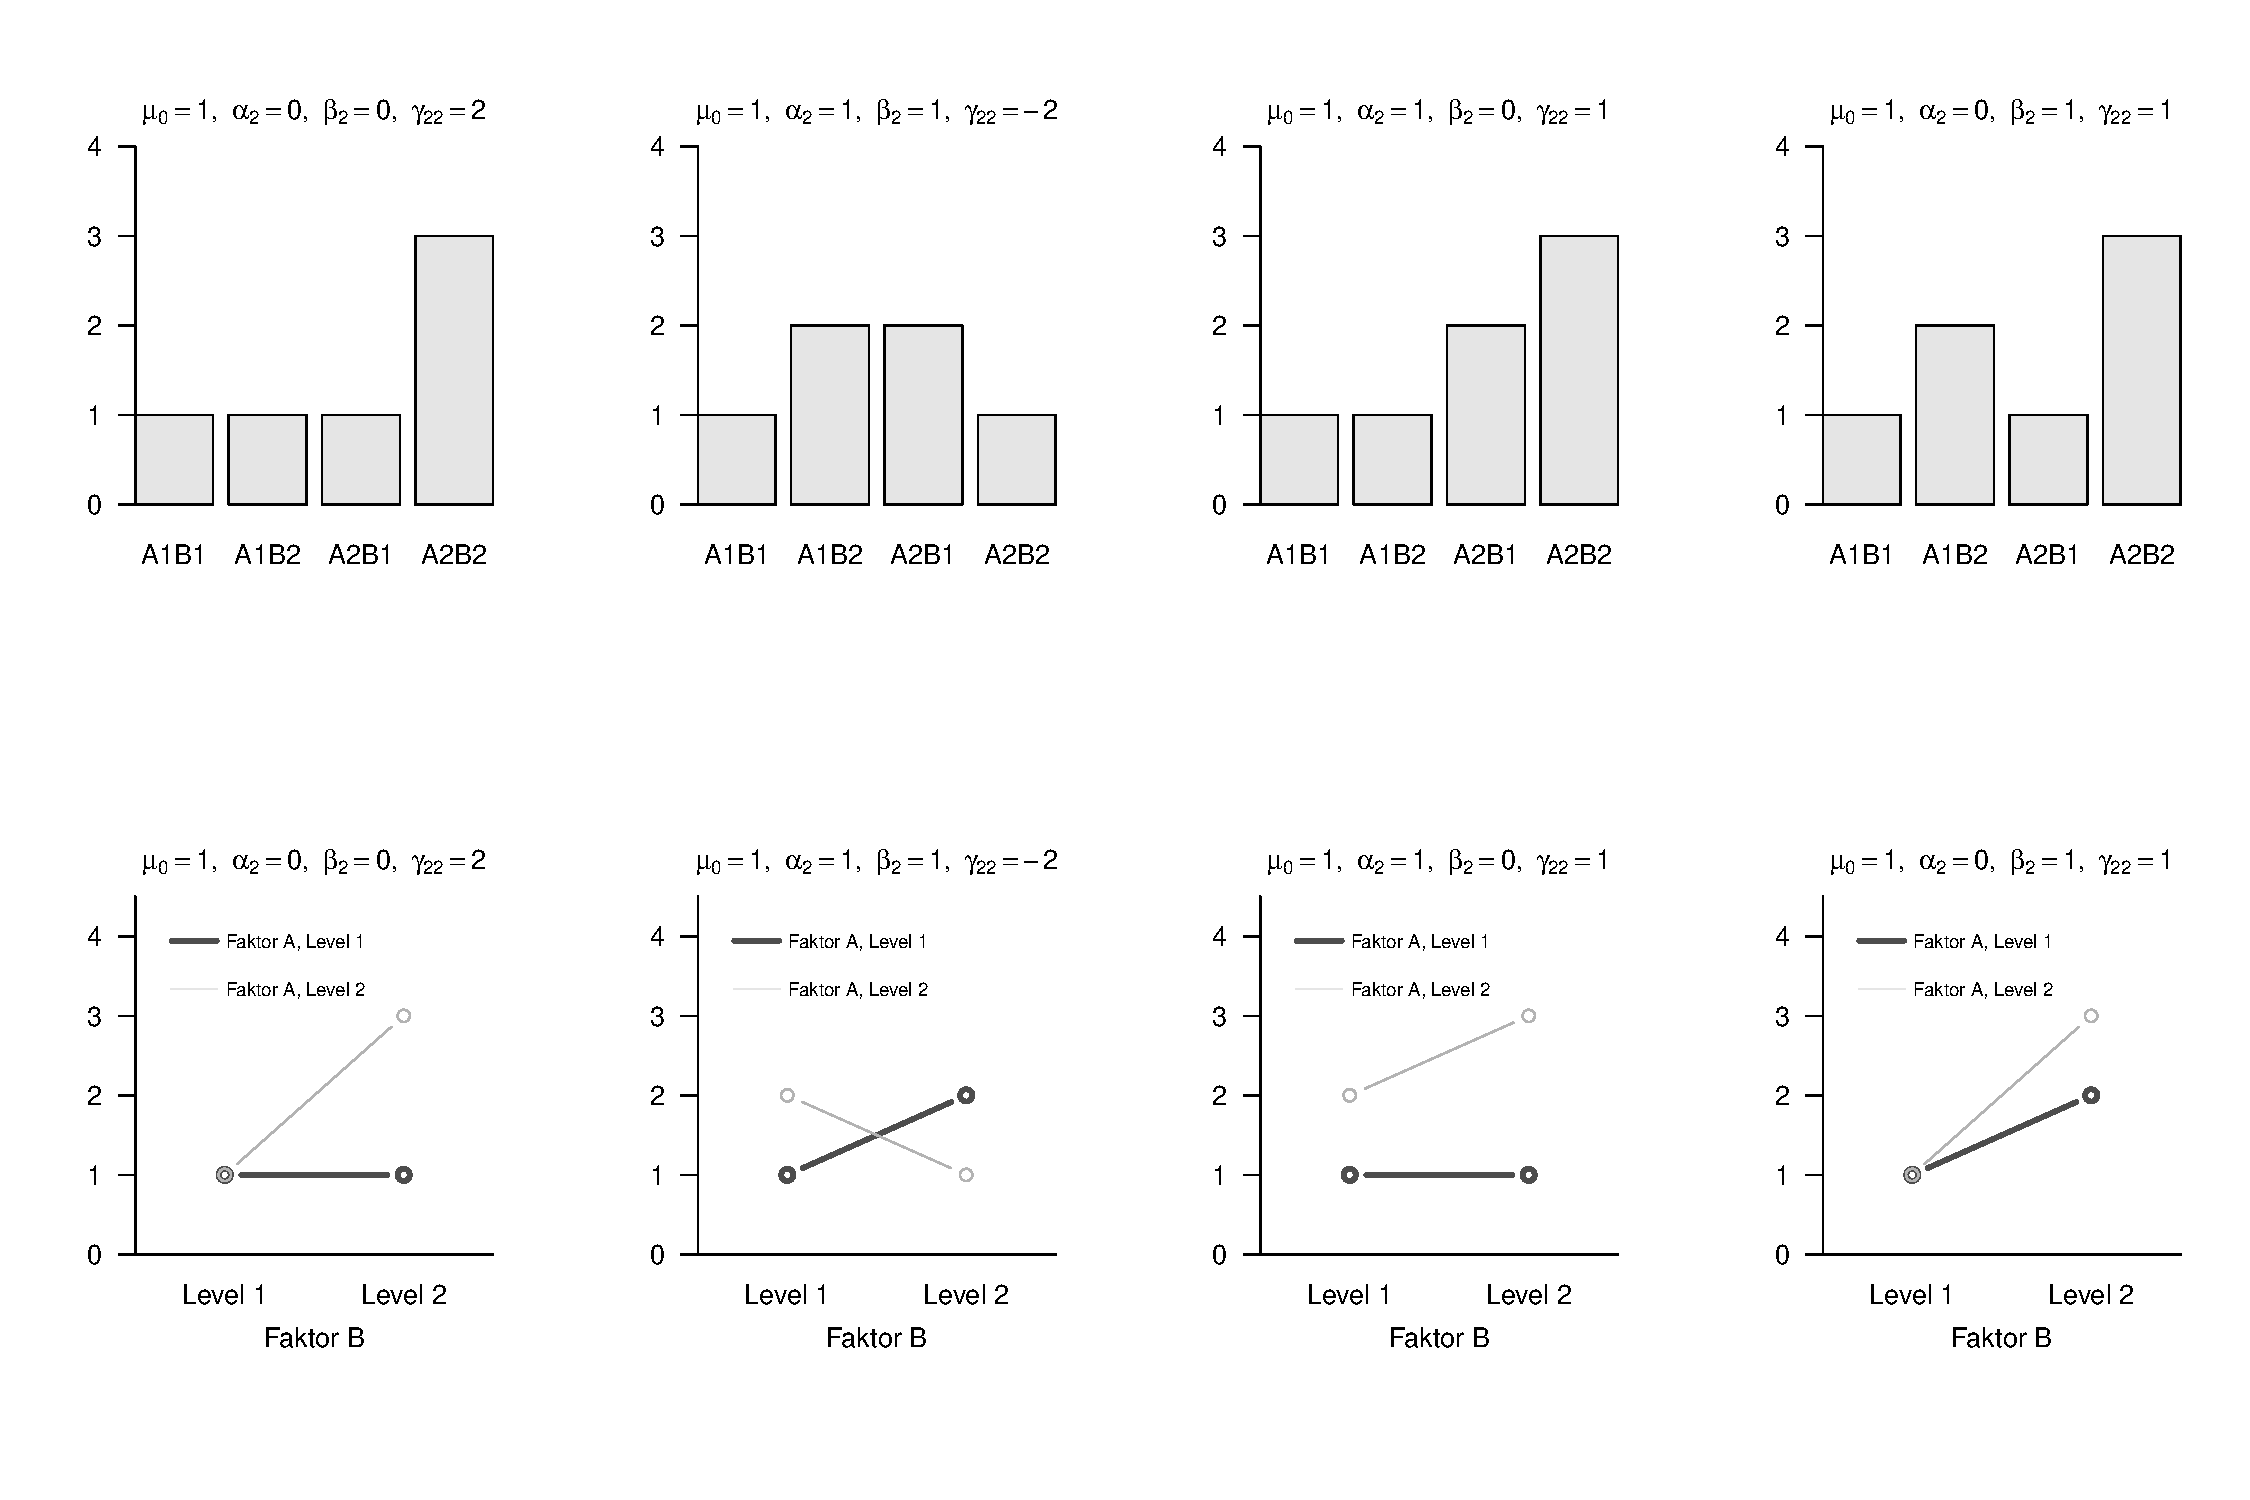
\includegraphics[width=1\linewidth]{11_Abbildungen/alm_11_zva_int_beispiel} \end{center}
\end{frame}

\begin{frame}{Modellformulierung}
\protect\hypertarget{modellformulierung-9}{}
\footnotesize
\setstretch{1.2}
\vspace{2mm}
\begin{theorem}[\small Designmatrixform des Modells der 2 x 2 ZVA mit Interaktion und Referenzgruppe]
\justifying
\normalfont
Gegeben sei die strukturelle Form eines 2 x 2 ZVA Modells mit Interaktion und Referenzgruppe
und es sei
\begin{equation}
n := \sum_{i=1}^2 \sum_{i=1}^2 n_{ij}
\end{equation}
die Gesamtanzahl an Datenvariablen. Dann hat dieses Modell die Designmatrixform
\begin{equation}
y \sim N(X\beta,\sigma^2I_n), \mbox{ mit }
\end{equation}
\begin{equation}
y:=
\begin{pmatrix}
y_{111}\\
\vdots \\
y_{11n_{11}}\\
y_{121}\\
\vdots \\
y_{12n_{12}}\\
y_{211}\\
\vdots \\
y_{21n_{21}}\\
y_{221}\\
\vdots \\
y_{22n_{22}}\\
\end{pmatrix}, \,
X =
\begin{pmatrix}
1       &   0       &   0        &  0       \\
\vdots  &   \vdots  &   \vdots   &  \vdots  \\
1       &   0       &   0        &  0       \\
1       &   0       &   1        &  0       \\
\vdots  &   \vdots  &   \vdots   &  \vdots  \\
1       &   0       &   1        &  0       \\
1       &   1       &   0        &  0       \\
\vdots  &   \vdots  &   \vdots   &  \vdots  \\
1       &   1       &   0        &  0       \\
1       &   1       &   1        &  1       \\
\vdots  &   \vdots  &   \vdots   &  \vdots  \\
1       &   1       &   1        &  1       \\
\end{pmatrix} \in \mathbb{R}^{n \times 4}, \,
\beta :=
\begin{pmatrix}
\mu_0               \\
\alpha_{2}          \\
\beta_{2}           \\
\gamma_{22}
\end{pmatrix}
\in \mathbb{R}^{4}
\mbox{ und }
\sigma^2 > 0.
\end{equation}
\end{theorem}
\end{frame}

\begin{frame}{Modellformulierung}
\protect\hypertarget{modellformulierung-10}{}
\textcolor{darkblue}{Beispiel}

\footnotesize

Es seien \begin{equation}
I := 2, J := 2 \mbox{ und } n_{ij} := 4 \mbox{ für } i = 1,2, j = 1,2 \mbox{, also } n = 16.
\end{equation} Dann gilt \begin{equation}
y = X\beta + \varepsilon \mbox{ mit } \varepsilon \sim N(0_{16},\sigma^2 I_{16})
\end{equation} mit \footnotesize \begin{equation}
y :=
\begin{pmatrix}
y_{111} \\
y_{112} \\
y_{113} \\
y_{114} \\
y_{121} \\
y_{122} \\
y_{123} \\
y_{124} \\
y_{211} \\
y_{212} \\
y_{213} \\
y_{214} \\
y_{221} \\
y_{222} \\
y_{223} \\
y_{224}
\end{pmatrix},
\,
X :=
\begin{pmatrix}
1  &  0  &   0   &  0  \\
1  &  0  &   0   &  0  \\
1  &  0  &   0   &  0  \\
1  &  0  &   0   &  0  \\
1  &  0  &   1   &  0  \\
1  &  0  &   1   &  0  \\
1  &  0  &   1   &  0  \\
1  &  0  &   1   &  0  \\
1  &  1  &   0   &  0  \\
1  &  1  &   0   &  0  \\
1  &  1  &   0   &  0  \\
1  &  1  &   0   &  0  \\
1  &  1  &   1   &  1  \\
1  &  1  &   1   &  1  \\
1  &  1  &   1   &  1  \\
1  &  1  &   1   &  1  \\
\end{pmatrix}
\in \mathbb{R}^{16 \times 4},
\,
\beta :=
\begin{pmatrix}
\mu_0       \\
\alpha_2    \\
\beta_2     \\
\gamma_{22} \\
\end{pmatrix}
\in \mathbb{R}^{4}
\mbox{ und }
\sigma^2 > 0.
\end{equation}
\end{frame}

\begin{frame}[fragile]{Modellformulierung}
\protect\hypertarget{modellformulierung-11}{}
\vspace{2mm}

\textcolor{darkblue}{Beispiel} \vspace{1mm} \tiny \setstretch{.85}

\begin{Shaded}
\begin{Highlighting}[]
\CommentTok{\# Modellformulierung}
\FunctionTok{library}\NormalTok{(MASS)                               }\CommentTok{\# Multivariate Normalverteilung}
\NormalTok{I      }\OtherTok{=} \DecValTok{2}                                  \CommentTok{\# Anzahl Level Faktor A}
\NormalTok{J      }\OtherTok{=} \DecValTok{2}                                  \CommentTok{\# Anzahl Level Faktor B}
\NormalTok{n\_ij   }\OtherTok{=} \DecValTok{4}                                  \CommentTok{\# Anzahl von Datenpunkten der i,jten Gruppe}
\NormalTok{n      }\OtherTok{=}\NormalTok{ I}\SpecialCharTok{*}\NormalTok{J}\SpecialCharTok{*}\NormalTok{n\_ij                           }\CommentTok{\# Anzahl Datenpunkte}
\NormalTok{p      }\OtherTok{=} \DecValTok{1} \SpecialCharTok{+}\NormalTok{ (I}\DecValTok{{-}1}\NormalTok{)}\SpecialCharTok{+}\NormalTok{(J}\DecValTok{{-}1}\NormalTok{)}\SpecialCharTok{+}\NormalTok{(I}\SpecialCharTok{*}\NormalTok{J}\DecValTok{{-}3}\NormalTok{)            }\CommentTok{\# Anzahl Parameter}
\NormalTok{D      }\OtherTok{=} \FunctionTok{matrix}\NormalTok{(}\FunctionTok{c}\NormalTok{(}\DecValTok{1}\NormalTok{,}\DecValTok{0}\NormalTok{,}\DecValTok{0}\NormalTok{,}\DecValTok{0}\NormalTok{,                  }\CommentTok{\# Prototypische Designmatrix für balancierte Designs}
                  \DecValTok{1}\NormalTok{,}\DecValTok{0}\NormalTok{,}\DecValTok{1}\NormalTok{,}\DecValTok{0}\NormalTok{,}
                  \DecValTok{1}\NormalTok{,}\DecValTok{1}\NormalTok{,}\DecValTok{0}\NormalTok{,}\DecValTok{0}\NormalTok{,}
                  \DecValTok{1}\NormalTok{,}\DecValTok{1}\NormalTok{,}\DecValTok{1}\NormalTok{,}\DecValTok{1}\NormalTok{),}
                \AttributeTok{nrow  =}\NormalTok{ p,}
                \AttributeTok{byrow =} \ConstantTok{TRUE}\NormalTok{)}
\NormalTok{C      }\OtherTok{=} \FunctionTok{matrix}\NormalTok{(}\FunctionTok{rep}\NormalTok{(}\DecValTok{1}\NormalTok{,n\_ij),}\AttributeTok{nrow =}\NormalTok{ n\_ij)    }\CommentTok{\# Prototypischer Zellenvektor für balancierte Designs}
\NormalTok{X      }\OtherTok{=} \FunctionTok{kronecker}\NormalTok{(D,C)                     }\CommentTok{\# Kroneckerprodukt Designmatrix Erzeugung für balancierte Designs}
\NormalTok{I\_n    }\OtherTok{=} \FunctionTok{diag}\NormalTok{(n)                            }\CommentTok{\# n x n Einheitsmatrix}
\NormalTok{beta   }\OtherTok{=} \FunctionTok{matrix}\NormalTok{(}\FunctionTok{c}\NormalTok{(}\DecValTok{1}\NormalTok{,}\DecValTok{1}\NormalTok{,}\DecValTok{1}\NormalTok{,}\DecValTok{1}\NormalTok{), }\AttributeTok{nrow =}\NormalTok{ p)       }\CommentTok{\# \textbackslash{}beta = (\textbackslash{}mu\_0,\textbackslash{}alpha\_2,\textbackslash{}alpha\_3,\textbackslash{}alpha\_4)}
\NormalTok{sigsqr }\OtherTok{=} \DecValTok{10}                                 \CommentTok{\# \textbackslash{}sigma\^{}2}

\CommentTok{\# Datenrealisierung}
\NormalTok{y      }\OtherTok{=} \FunctionTok{mvrnorm}\NormalTok{(}\DecValTok{1}\NormalTok{, X }\SpecialCharTok{\%*\%}\NormalTok{ beta, sigsqr}\SpecialCharTok{*}\NormalTok{I\_n) }\CommentTok{\# eine Realisierung eines n{-}dimensionalen ZVs}
\FunctionTok{print}\NormalTok{(X)}
\end{Highlighting}
\end{Shaded}

\begin{verbatim}
>       [,1] [,2] [,3] [,4]
>  [1,]    1    0    0    0
>  [2,]    1    0    0    0
>  [3,]    1    0    0    0
>  [4,]    1    0    0    0
>  [5,]    1    0    1    0
>  [6,]    1    0    1    0
>  [7,]    1    0    1    0
>  [8,]    1    0    1    0
>  [9,]    1    1    0    0
> [10,]    1    1    0    0
> [11,]    1    1    0    0
> [12,]    1    1    0    0
> [13,]    1    1    1    1
> [14,]    1    1    1    1
> [15,]    1    1    1    1
> [16,]    1    1    1    1
\end{verbatim}
\end{frame}

\begin{frame}[fragile]{Modellformulierung}
\protect\hypertarget{modellformulierung-12}{}
\vspace{2mm}

\textcolor{darkblue}{Beispieldatensatzerzeugung} \vspace{1mm} \tiny
\setstretch{1}

\begin{Shaded}
\begin{Highlighting}[]
\CommentTok{\# Datensimulation}
\FunctionTok{library}\NormalTok{(MASS)                                            }\CommentTok{\# Multivariate Normalverteilung}
\FunctionTok{set.seed}\NormalTok{(}\DecValTok{1}\NormalTok{)                                              }\CommentTok{\# reproduzierbare Daten}
\NormalTok{I             }\OtherTok{=} \DecValTok{2}                                        \CommentTok{\# Anzahl Level Faktor A (Therapie)}
\NormalTok{J             }\OtherTok{=} \DecValTok{2}                                        \CommentTok{\# Anzahl Level Faktor B (Alter)}
\NormalTok{n\_ij          }\OtherTok{=} \DecValTok{20}                                       \CommentTok{\# Anzahl von Datenpunkten der i,jten Gruppe}
\NormalTok{n             }\OtherTok{=}\NormalTok{ I}\SpecialCharTok{*}\NormalTok{J}\SpecialCharTok{*}\NormalTok{n\_ij                                 }\CommentTok{\# Anzahl Datenpunkte}
\NormalTok{p             }\OtherTok{=} \DecValTok{1} \SpecialCharTok{+}\NormalTok{ (I}\DecValTok{{-}1}\NormalTok{)}\SpecialCharTok{+}\NormalTok{(J}\DecValTok{{-}1}\NormalTok{)}\SpecialCharTok{+}\NormalTok{(I}\SpecialCharTok{*}\NormalTok{J}\DecValTok{{-}3}\NormalTok{)                  }\CommentTok{\# Anzahl Parameter}
\NormalTok{D             }\OtherTok{=} \FunctionTok{matrix}\NormalTok{(}\FunctionTok{c}\NormalTok{(}\DecValTok{1}\NormalTok{,}\DecValTok{0}\NormalTok{,}\DecValTok{0}\NormalTok{,}\DecValTok{0}\NormalTok{,                        }\CommentTok{\# Prototypische Designmatrix für balancierte Designs}
                         \DecValTok{1}\NormalTok{,}\DecValTok{0}\NormalTok{,}\DecValTok{1}\NormalTok{,}\DecValTok{0}\NormalTok{,}
                         \DecValTok{1}\NormalTok{,}\DecValTok{1}\NormalTok{,}\DecValTok{0}\NormalTok{,}\DecValTok{0}\NormalTok{,}
                         \DecValTok{1}\NormalTok{,}\DecValTok{1}\NormalTok{,}\DecValTok{1}\NormalTok{,}\DecValTok{1}\NormalTok{),}
                \AttributeTok{nrow  =}\NormalTok{ p,}
                \AttributeTok{byrow =} \ConstantTok{TRUE}\NormalTok{)}
\NormalTok{C             }\OtherTok{=} \FunctionTok{matrix}\NormalTok{(}\FunctionTok{rep}\NormalTok{(}\DecValTok{1}\NormalTok{,n\_ij),}\AttributeTok{nrow =}\NormalTok{ n\_ij)          }\CommentTok{\# Prototypischer Zellenvektor für balancierte Designs}
\NormalTok{X             }\OtherTok{=} \FunctionTok{kronecker}\NormalTok{(D,C)                           }\CommentTok{\# Kroneckerprodukt für balancierte Designs}
\NormalTok{I\_n           }\OtherTok{=} \FunctionTok{diag}\NormalTok{(n)                                  }\CommentTok{\# n x n Einheitsmatrix}
\NormalTok{beta          }\OtherTok{=} \FunctionTok{matrix}\NormalTok{(}\FunctionTok{c}\NormalTok{(}\DecValTok{7}\NormalTok{,}\SpecialCharTok{{-}}\DecValTok{3}\NormalTok{,}\DecValTok{0}\NormalTok{,}\SpecialCharTok{{-}}\DecValTok{2}\NormalTok{), }\AttributeTok{nrow =}\NormalTok{ p)           }\CommentTok{\# \textbackslash{}beta = (\textbackslash{}mu\_0,\textbackslash{}alpha\_2,\textbackslash{}beta\_2,\textbackslash{}gamma\_22)}
\NormalTok{sigsqr        }\OtherTok{=} \DecValTok{4}                                        \CommentTok{\# \textbackslash{}sigma\^{}2}
\NormalTok{y             }\OtherTok{=} \FunctionTok{mvrnorm}\NormalTok{(}\DecValTok{1}\NormalTok{, X }\SpecialCharTok{\%*\%}\NormalTok{ beta, sigsqr}\SpecialCharTok{*}\NormalTok{I\_n)       }\CommentTok{\# eine Realisierung eines n{-}dimensionalen ZVs}

\CommentTok{\# Dataframeformatierung}
\FunctionTok{library}\NormalTok{(writexl)                                         }\CommentTok{\# Excel Output}
\NormalTok{D            }\OtherTok{=} \FunctionTok{data.frame}\NormalTok{(}\StringTok{"ID"} \OtherTok{=} \DecValTok{1}\SpecialCharTok{:}\NormalTok{n)                    }\CommentTok{\# Dataframe Initialisierung und ID Variable}
\NormalTok{D}\SpecialCharTok{$}\NormalTok{Therapy    }\OtherTok{=} \FunctionTok{c}\NormalTok{(}\FunctionTok{rep}\NormalTok{(}\StringTok{"F2F"}\NormalTok{, J}\SpecialCharTok{*}\NormalTok{n\_ij), }\FunctionTok{rep}\NormalTok{(}\StringTok{"ONL"}\NormalTok{, J}\SpecialCharTok{*}\NormalTok{n\_ij)) }\CommentTok{\# Therapiebedingung}
\NormalTok{D}\SpecialCharTok{$}\NormalTok{Age        }\OtherTok{=} \FunctionTok{rep}\NormalTok{(}\FunctionTok{c}\NormalTok{(}\FunctionTok{rep}\NormalTok{(}\StringTok{"YA"}\NormalTok{, n\_ij), }\FunctionTok{rep}\NormalTok{(}\StringTok{"OA"}\NormalTok{,n\_ij)),I) }\CommentTok{\# Alter}
\NormalTok{D}\SpecialCharTok{$}\NormalTok{BDI        }\OtherTok{=}\NormalTok{ y                                         }\CommentTok{\# PrePost{-}BDI Differenzwerte}

\CommentTok{\# Datenspeicherung}
\FunctionTok{write\_xlsx}\NormalTok{(D, }\FunctionTok{file.path}\NormalTok{(}\FunctionTok{getwd}\NormalTok{()       , }\StringTok{"11\_Daten"}\NormalTok{, }\StringTok{"11\_Zweifaktorielle\_Varianzanalyse\_Daten.xlsx"}\NormalTok{))}
\FunctionTok{write.csv}\NormalTok{( D, }\AttributeTok{file =} \FunctionTok{file.path}\NormalTok{(}\FunctionTok{getwd}\NormalTok{(), }\StringTok{"11\_Daten"}\NormalTok{, }\StringTok{"11\_Zweifaktorielle\_Varianzanalyse\_Daten.csv"}\NormalTok{))}
\end{Highlighting}
\end{Shaded}
\end{frame}

\begin{frame}{}
\protect\hypertarget{section-6}{}
\large
\setstretch{2.7}
\vfill

Anwendungsszenario

Modellformulierung

\textbf{Modellschätzung}

Modellevaluation

Selbstkontrollfragen \vfill
\end{frame}

\begin{frame}{Modellschätzung}
\protect\hypertarget{modellschuxe4tzung}{}
\footnotesize
\begin{theorem}[\begin{small} Betaparameterschätzung im additiven 2 x 2 ZVA Modell mit Referenzgruppe \end{small}]
\justifying
\normalfont
Gegeben sei die Designmatrixform eines balancierten additiven 2 x 2 ZVA Modells mit
Referenzgruppe. Dann ergibt sich für den Betaparameterschätzer
\begin{equation}
\hat{\beta} :=
\begin{pmatrix}
\hat{\mu}_0       \\
\hat{\alpha}_2    \\
\hat{\beta}_2     \\
\end{pmatrix}
=
\begin{pmatrix}
\frac{3}{4}\bar{y}_{11} + \frac{1}{4}(\bar{y}_{12} + \bar{y}_{21}) - \frac{1}{4}\bar{y}_{22} \\
\frac{1}{2}(\bar{y}_{21} + \bar{y}_{22}) - \frac{1}{2}(\bar{y}_{11} + \bar{y}_{12})           \\
\frac{1}{2}(\bar{y}_{12} + \bar{y}_{22}) - \frac{1}{2}(\bar{y}_{11} + \bar{y}_{21})           \\
\end{pmatrix},
\end{equation}
wobei
\begin{equation}
\bar{y}_{ij} := \frac{1}{n_{ij}}\sum_{k = 1}^{n_{ij}} y_{ijk} \mbox{ für } 1 \le i,j \le 2
\end{equation}
das Stichprobenmittel der $i,j$ten Gruppe des 2 x 2 ZVA Designs bezeichnet.
\end{theorem}

\footnotesize

\underline{Beweis}

Wir bestimmen zunächst \(X^Ty, X^TX\) und \((X^TX)^{-1}\) bei konstantem
\(n_{ij}\) für \(1 \le i,j \le 2\).
\end{frame}

\begin{frame}{Modellschätzung}
\protect\hypertarget{modellschuxe4tzung-1}{}
\footnotesize
\vspace{1mm}

\underline{Beweis (fortgeführt)}

\tiny

\begin{align}
\renewcommand{\arraystretch}{1.2}
\begin{split}
X^Ty
& =
\setcounter{MaxMatrixCols}{20}
\begin{pmatrix}
1 & \cdots & 1 & 1 & \cdots & 1 & 1 & \cdots & 1 & 1 & \cdots & 1   \\
0 & \cdots & 0 & 0 & \cdots & 0 & 1 & \cdots & 1 & 1 & \cdots & 1   \\
0 & \cdots & 0 & 1 & \cdots & 1 & 0 & \cdots & 0 & 1 & \cdots & 1   \\
\end{pmatrix}
\begin{pmatrix*}[l]
y_{111}     \\  \vdots  \\ y_{11n_{11}}
\\
y_{121}     \\  \vdots  \\ y_{12n_{12}}
\\
y_{211}     \\  \vdots  \\ y_{21n_{21}}
\\
y_{221}     \\  \vdots  \\ y_{22n_{22}}
\end{pmatrix*}
\\
& =
\begin{pmatrix*}[l]
\sum_{i=1}^2 \sum_{j=1}^2 \sum_{k = 1}^{n_{ij}} y_{ijk}     \\
\sum_{j=1}^2 \sum_{k = 1}^{n_{2j}} y_{2jk}                  \\
\sum_{i=1}^2 \sum_{k = 1}^{n_{i2}} y_{i2k}                  \\
\end{pmatrix*}.
\end{split}
\end{align}
\end{frame}

\begin{frame}{Modellschätzung}
\protect\hypertarget{modellschuxe4tzung-2}{}
\footnotesize
\vspace{1mm}

\underline{Beweis (fortgeführt)}

\tiny

\begin{align}
\renewcommand{\arraystretch}{1}
\begin{split}
X^TX
& =
\setcounter{MaxMatrixCols}{20}
\begin{pmatrix}
1 & \cdots & 1 & 1 & \cdots & 1 & 1 & \cdots & 1 & 1 & \cdots & 1   \\
0 & \cdots & 0 & 0 & \cdots & 0 & 1 & \cdots & 1 & 1 & \cdots & 1   \\
0 & \cdots & 0 & 1 & \cdots & 1 & 0 & \cdots & 0 & 1 & \cdots & 1   \\
\end{pmatrix}
\begin{pmatrix}
1       &   0       &   0        \\
\vdots  &   \vdots  &   \vdots   \\
1       &   0       &   0        \\
1       &   0       &   1        \\
\vdots  &   \vdots  &   \vdots   \\
1       &   0       &   1        \\
1       &   1       &   0        \\
\vdots  &   \vdots  &   \vdots   \\
1       &   1       &   0        \\
1       &   1       &   1        \\
\vdots  &   \vdots  &   \vdots   \\
1       &   1       &   1        \\
\end{pmatrix}
\\
&
=
n_{ij}
\begin{pmatrix*}[r]
4 & 2 & 2 \\
2 & 2 & 1 \\
2 & 1 & 2 \\
\end{pmatrix*}
\end{split}
\end{align}
\end{frame}

\begin{frame}{Modellschätzung}
\protect\hypertarget{modellschuxe4tzung-3}{}
\footnotesize
\vspace{1mm}

\underline{Beweis (fortgeführt)}

Ohne Beweis halten wir weiterhin fest, dass

\begin{align}
(X^T X)^{-1}
=
n_{ij}
\begin{pmatrix*}[r]
4 & 2 & 2 \\
2 & 2 & 1 \\
2 & 1 & 2\\
\end{pmatrix*}^{-1}
=
\frac{1}{n_{ij}}
\begin{pmatrix*}[r]
 \frac{3}{4} & -\frac{1}{2} & -\frac{1}{2} \\
-\frac{1}{2} & 1            & 0            \\
-\frac{1}{2} & 0            & 1            \\
\end{pmatrix*}
\end{align}

Es ergibt sich also \begin{equation}
\hat{\beta}
=
\begin{pmatrix}
\hat{\mu}_0      \\
\hat{\alpha}_2   \\
\hat{\beta}_2    \\
\end{pmatrix}
=
\frac{1}{n_{ij}}
\begin{pmatrix*}[r]
 \frac{3}{4} & -\frac{1}{2} & -\frac{1}{2} \\
-\frac{1}{2} & 1            & 0            \\
-\frac{1}{2} & 0            & 1            \\
\end{pmatrix*}
\begin{pmatrix*}[l]
\sum_{i=1}^2 \sum_{j=1}^2 \sum_{k = 1}^{n_{ij}} y_{ijk}     \\
\sum_{j=1}^2 \sum_{k = 1}^{n_{2j}} y_{2jk}                  \\
\sum_{i=1}^2 \sum_{k = 1}^{n_{i2}} y_{i2k}                  \\
\end{pmatrix*}.
\end{equation}
\end{frame}

\begin{frame}{Modellschätzung}
\protect\hypertarget{modellschuxe4tzung-4}{}
\footnotesize

\underline{Beweis (fortgeführt)}

Damit ergibt sich dann \tiny \begin{align}
\begin{split}
\hat{\mu}_0
& =
\frac{1}{n_{ij}}
\left(
  \frac{3}{4}\sum_{i=1}^2 \sum_{j=1}^2 \sum_{k = 1}^{n_{ij}} y_{ijk}
- \frac{1}{2}\sum_{j=1}^2 \sum_{k = 1}^{n_{2j}} y_{2jk}
- \frac{1}{2}\sum_{i=1}^2 \sum_{k = 1}^{n_{i2}} y_{i2k}
\right)
\\
& =
\frac{1}{n_{ij}}
\left(
  \frac{3}{4}\sum_{k = 1}^{n_{11}} y_{11k}
+ \frac{3}{4}\sum_{k = 1}^{n_{12}} y_{12k}
+ \frac{3}{4}\sum_{k = 1}^{n_{21}} y_{21k}
+ \frac{3}{4}\sum_{k = 1}^{n_{22}} y_{22k}
\right)
\\
&
+ \frac{1}{n_{ij}}
\left(
- \frac{1}{2}\sum_{k = 1}^{n_{21}} y_{21k} - \frac{1}{2}\sum_{k = 1}^{n_{22}} y_{22k}
- \frac{1}{2}\sum_{k = 1}^{n_{12}} y_{12k} - \frac{1}{2}\sum_{k = 1}^{n_{22}} y_{22k}
\right)
\\
& = \frac{1}{n_{ij}}
\left(
  \frac{3}{4}\sum_{k = 1}^{n_{11}} y_{11k}
+ \frac{1}{4}\sum_{k = 1}^{n_{12}} y_{12k}
+ \frac{1}{4}\sum_{k = 1}^{n_{21}} y_{21k}
- \frac{1}{4}\sum_{k = 1}^{n_{22}} y_{22k}
\right)
\\
& =
  \frac{3}{4}\bar{y}_{11}
+ \frac{1}{4}(\bar{y}_{12} + \bar{y}_{21})
- \frac{1}{4}\bar{y}_{22}
\end{split}
\end{align}
\end{frame}

\begin{frame}{Modellschätzung}
\protect\hypertarget{modellschuxe4tzung-5}{}
\footnotesize

\underline{Beweis (fortgeführt)}

sowie \tiny \begin{align}
\begin{split}
\hat{\alpha}_2
& =
\frac{1}{n_{ij}}
\left(
- \frac{1}{2} \sum_{i=1}^2 \sum_{j=1}^2 \sum_{k = 1}^{n_{ij}} y_{ijk} + \sum_{j=1}^2 \sum_{k = 1}^{n_{2j}} y_{2jk}
\right)
\\
& =
\frac{1}{n_{ij}}
\left(
- \frac{1}{2}\sum_{k = 1}^{n_{11}} y_{11k}
- \frac{1}{2}\sum_{k = 1}^{n_{12}} y_{12k}
- \frac{1}{2}\sum_{k = 1}^{n_{21}} y_{21k}
- \frac{1}{2}\sum_{k = 1}^{n_{22}} y_{22k}
+            \sum_{k = 1}^{n_{21}} y_{21k}
+            \sum_{k = 1}^{n_{22}} y_{22k}
\right)
\\
& =
\frac{1}{n_{ij}}
\left(
- \frac{1}{2}\sum_{k = 1}^{n_{11}} y_{11k}
- \frac{1}{2}\sum_{k = 1}^{n_{12}} y_{12k}
+ \frac{1}{2}\sum_{k = 1}^{n_{21}} y_{21k}
+ \frac{1}{2}\sum_{k = 1}^{n_{22}} y_{22k}
\right)
\\
& = \frac{1}{2}(\bar{y}_{21} + \bar{y}_{22}) - \frac{1}{2}(\bar{y}_{11} + \bar{y}_{12})
\end{split}
\end{align} \footnotesize und analog für \(\hat{\beta}_2\).
\end{frame}

\begin{frame}[fragile]{Modellschätzung}
\protect\hypertarget{modellschuxe4tzung-6}{}
\vspace{2mm}

\textcolor{darkblue}{Beispiel} \tiny \vspace{1mm} \setstretch{.6}

\begin{Shaded}
\begin{Highlighting}[]
\CommentTok{\# Datenreformatierung}
\NormalTok{fname      }\OtherTok{=} \FunctionTok{file.path}\NormalTok{(}\FunctionTok{getwd}\NormalTok{(), }\StringTok{"11\_Daten"}\NormalTok{, }\StringTok{"11\_Zweifaktorielle\_Varianzanalyse\_Daten.csv"}\NormalTok{)}
\NormalTok{D          }\OtherTok{=} \FunctionTok{read.table}\NormalTok{(fname, }\AttributeTok{sep =} \StringTok{","}\NormalTok{, }\AttributeTok{header =} \ConstantTok{TRUE}\NormalTok{)     }\CommentTok{\# Datensatz}
\NormalTok{A1B1       }\OtherTok{=}\NormalTok{ D}\SpecialCharTok{$}\NormalTok{BDI[D}\SpecialCharTok{$}\NormalTok{Therapy }\SpecialCharTok{==} \StringTok{"F2F"} \SpecialCharTok{\&}\NormalTok{ D}\SpecialCharTok{$}\NormalTok{Age }\SpecialCharTok{==} \StringTok{"YA"}\NormalTok{ ]      }\CommentTok{\# Face{-}to{-}face, younger adults}
\NormalTok{A1B2       }\OtherTok{=}\NormalTok{ D}\SpecialCharTok{$}\NormalTok{BDI[D}\SpecialCharTok{$}\NormalTok{Therapy }\SpecialCharTok{==} \StringTok{"F2F"} \SpecialCharTok{\&}\NormalTok{ D}\SpecialCharTok{$}\NormalTok{Age }\SpecialCharTok{==} \StringTok{"OA"}\NormalTok{ ]      }\CommentTok{\# Face{-}to{-}face, younger adults}
\NormalTok{A2B1       }\OtherTok{=}\NormalTok{ D}\SpecialCharTok{$}\NormalTok{BDI[D}\SpecialCharTok{$}\NormalTok{Therapy }\SpecialCharTok{==} \StringTok{"ONL"} \SpecialCharTok{\&}\NormalTok{ D}\SpecialCharTok{$}\NormalTok{Age }\SpecialCharTok{==} \StringTok{"YA"}\NormalTok{ ]      }\CommentTok{\# Online,       older   adults}
\NormalTok{A2B2       }\OtherTok{=}\NormalTok{ D}\SpecialCharTok{$}\NormalTok{BDI[D}\SpecialCharTok{$}\NormalTok{Therapy }\SpecialCharTok{==} \StringTok{"ONL"} \SpecialCharTok{\&}\NormalTok{ D}\SpecialCharTok{$}\NormalTok{Age }\SpecialCharTok{==} \StringTok{"OA"}\NormalTok{ ]      }\CommentTok{\# Online,       older   adults}

\CommentTok{\# Datenmatrix für Gruppenmittelwerte}
\NormalTok{n\_ij       }\OtherTok{=} \FunctionTok{length}\NormalTok{(A1B1)                                    }\CommentTok{\# Anzahl Datenpunkte pro Gruppe}
\NormalTok{Y          }\OtherTok{=} \FunctionTok{matrix}\NormalTok{(}\FunctionTok{c}\NormalTok{(A1B1,A1B2,A2B1,A2B2), }\AttributeTok{nrow =}\NormalTok{ n\_ij)     }\CommentTok{\# Datenmatrix}
\NormalTok{bar\_y      }\OtherTok{=} \FunctionTok{colMeans}\NormalTok{(Y)                                     }\CommentTok{\# Zellenmittelwerte}

\CommentTok{\# Modellschätzung}
\NormalTok{I          }\OtherTok{=} \DecValTok{2}                                               \CommentTok{\# Anzahl Level Faktor A (Therapie)}
\NormalTok{J          }\OtherTok{=} \DecValTok{2}                                               \CommentTok{\# Anzahl Level Faktor B (Alter)}
\NormalTok{n          }\OtherTok{=}\NormalTok{ I}\SpecialCharTok{*}\NormalTok{J}\SpecialCharTok{*}\NormalTok{n\_ij                                        }\CommentTok{\# Anzahl Datenpunkte}
\NormalTok{p          }\OtherTok{=} \DecValTok{1} \SpecialCharTok{+}\NormalTok{ (I}\DecValTok{{-}1}\NormalTok{)}\SpecialCharTok{+}\NormalTok{(J}\DecValTok{{-}1}\NormalTok{)}\SpecialCharTok{+}\NormalTok{(I}\SpecialCharTok{*}\NormalTok{J}\DecValTok{{-}3}\NormalTok{)                         }\CommentTok{\# Anzahl Parameter}
\NormalTok{D          }\OtherTok{=} \FunctionTok{matrix}\NormalTok{(}\FunctionTok{c}\NormalTok{(}\DecValTok{1}\NormalTok{,}\DecValTok{0}\NormalTok{,}\DecValTok{0}\NormalTok{,                                 }\CommentTok{\# Prototypische Designmatrix für balancierte Designs}
                      \DecValTok{1}\NormalTok{,}\DecValTok{0}\NormalTok{,}\DecValTok{1}\NormalTok{,}
                      \DecValTok{1}\NormalTok{,}\DecValTok{1}\NormalTok{,}\DecValTok{0}\NormalTok{,}
                      \DecValTok{1}\NormalTok{,}\DecValTok{1}\NormalTok{,}\DecValTok{1}\NormalTok{), }\AttributeTok{nrow =}\NormalTok{ p, }\AttributeTok{byrow =} \ConstantTok{TRUE}\NormalTok{)}
\NormalTok{C          }\OtherTok{=} \FunctionTok{matrix}\NormalTok{(}\FunctionTok{rep}\NormalTok{(}\DecValTok{1}\NormalTok{,n\_ij),}\AttributeTok{nrow =}\NormalTok{ n\_ij)                 }\CommentTok{\# Prototypischer Zellenvektor für balancierte Designs}
\NormalTok{X          }\OtherTok{=} \FunctionTok{kronecker}\NormalTok{(D,C)                                  }\CommentTok{\# Kroneckerprodukt Designmatrix}
\NormalTok{y          }\OtherTok{=} \FunctionTok{matrix}\NormalTok{(}\FunctionTok{c}\NormalTok{(A1B1,A1B2,A2B1,A2B2), }\AttributeTok{nrow =}\NormalTok{ n)        }\CommentTok{\# Datenvektor}
\NormalTok{beta\_hat   }\OtherTok{=} \FunctionTok{solve}\NormalTok{(}\FunctionTok{t}\NormalTok{(X) }\SpecialCharTok{\%*\%}\NormalTok{ X) }\SpecialCharTok{\%*\%} \FunctionTok{t}\NormalTok{(X) }\SpecialCharTok{\%*\%}\NormalTok{ y                }\CommentTok{\# Betaparameterschätzer}
\NormalTok{eps\_hat    }\OtherTok{=}\NormalTok{ y }\SpecialCharTok{{-}}\NormalTok{ X }\SpecialCharTok{\%*\%}\NormalTok{ beta\_hat                              }\CommentTok{\# Residuenvektor}
\NormalTok{sigsqr\_hat }\OtherTok{=}\NormalTok{ (}\FunctionTok{t}\NormalTok{(eps\_hat) }\SpecialCharTok{\%*\%}\NormalTok{ eps\_hat) }\SpecialCharTok{/}\NormalTok{(n}\SpecialCharTok{{-}}\NormalTok{p)                 }\CommentTok{\# Varianzparameterschätzer}
\FunctionTok{cat}\NormalTok{(}\StringTok{"hat\{beta\}                            : "}\NormalTok{   , beta\_hat,  }\CommentTok{\# Ausgabe}
    \StringTok{"}\SpecialCharTok{\textbackslash{}n}\StringTok{hat\{sigsqr\}                          : "}\NormalTok{ , sigsqr\_hat,}
    \StringTok{"}\SpecialCharTok{\textbackslash{}n}\StringTok{y\_11,y\_12,y\_21,y\_22                  : "}\NormalTok{ , bar\_y,}
    \StringTok{"}\SpecialCharTok{\textbackslash{}n}\StringTok{3/4y\_11 + 1/4(y\_12 + y\_21) {-} 1/4y\_22 : "}\NormalTok{ , (}\DecValTok{3}\SpecialCharTok{/}\DecValTok{4}\NormalTok{)}\SpecialCharTok{*}\NormalTok{bar\_y[}\DecValTok{1}\NormalTok{]}\SpecialCharTok{+}\NormalTok{(}\DecValTok{1}\SpecialCharTok{/}\DecValTok{4}\NormalTok{)}\SpecialCharTok{*}\NormalTok{(bar\_y[}\DecValTok{2}\NormalTok{]}\SpecialCharTok{+}\NormalTok{bar\_y[}\DecValTok{3}\NormalTok{])}\SpecialCharTok{{-}}\NormalTok{(}\DecValTok{1}\SpecialCharTok{/}\DecValTok{4}\NormalTok{)}\SpecialCharTok{*}\NormalTok{bar\_y[}\DecValTok{4}\NormalTok{],}
    \StringTok{"}\SpecialCharTok{\textbackslash{}n}\StringTok{1/2(y\_21 + y\_22) {-} 1/2(y\_11 + y\_12)  : "}\NormalTok{ , (}\DecValTok{1}\SpecialCharTok{/}\DecValTok{2}\NormalTok{)}\SpecialCharTok{*}\NormalTok{(bar\_y[}\DecValTok{3}\NormalTok{]}\SpecialCharTok{+}\NormalTok{bar\_y[}\DecValTok{4}\NormalTok{])}\SpecialCharTok{{-}}\NormalTok{(}\DecValTok{1}\SpecialCharTok{/}\DecValTok{2}\NormalTok{)}\SpecialCharTok{*}\NormalTok{(bar\_y[}\DecValTok{1}\NormalTok{] }\SpecialCharTok{+}\NormalTok{ bar\_y[}\DecValTok{2}\NormalTok{]),}
    \StringTok{"}\SpecialCharTok{\textbackslash{}n}\StringTok{1/2(y\_12 + y\_22) {-} 1/2(y\_11 + y\_21)  : "}\NormalTok{ , (}\DecValTok{1}\SpecialCharTok{/}\DecValTok{2}\NormalTok{)}\SpecialCharTok{*}\NormalTok{(bar\_y[}\DecValTok{2}\NormalTok{]}\SpecialCharTok{+}\NormalTok{bar\_y[}\DecValTok{4}\NormalTok{])}\SpecialCharTok{{-}}\NormalTok{(}\DecValTok{1}\SpecialCharTok{/}\DecValTok{2}\NormalTok{)}\SpecialCharTok{*}\NormalTok{(bar\_y[}\DecValTok{1}\NormalTok{] }\SpecialCharTok{+}\NormalTok{ bar\_y[}\DecValTok{3}\NormalTok{]))}
\end{Highlighting}
\end{Shaded}

\begin{verbatim}
> hat{beta}                            :  7.62 -4.06 -0.766 
> hat{sigsqr}                          :  3.54 
> y_11,y_12,y_21,y_22                  :  7.2 7.28 3.99 2.38 
> 3/4y_11 + 1/4(y_12 + y_21) - 1/4y_22 :  7.62 
> 1/2(y_21 + y_22) - 1/2(y_11 + y_12)  :  -4.06 
> 1/2(y_12 + y_22) - 1/2(y_11 + y_21)  :  -0.766
\end{verbatim}
\end{frame}

\begin{frame}{Modellschätzung}
\protect\hypertarget{modellschuxe4tzung-7}{}
\footnotesize
\begin{theorem}[\begin{small} Betaparameterschätzung im 2 x 2 ZVA Modell mit Interaktion und Referenzgruppe \end{small}]
\justifying
\normalfont
Gegeben sei die Designmatrixform eines balancierten 2 x 2 ZVA Modells mit
Interaktion und Referenzgruppe. Dann ergibt sich für den Betaparameterschätzer
\begin{equation}
\hat{\beta} :=
\begin{pmatrix}
\hat{\mu}_0       \\
\hat{\alpha}_2    \\
\hat{\beta}_2     \\
\hat{\gamma}_{22} \\
\end{pmatrix}
=
\begin{pmatrix}
\bar{y}_{11} \\
\bar{y}_{21} - \bar{y}_{11} \\
\bar{y}_{12} - \bar{y}_{11} \\
\bar{y}_{11} + \bar{y}_{22} - \bar{y}_{12} - \bar{y}_{21}  \\
\end{pmatrix},
\end{equation}
wobei
\begin{equation}
\bar{y}_{ij} := \frac{1}{n_{ij}}\sum_{k = 1}^{n_{ij}} y_{ijk} \mbox{ für } 1 \le i,j \le 2
\end{equation}
das Stichprobenmittel der $i,j$ten Gruppe des 2 x 2 ZVA Designs bezeichnet.
\end{theorem}

\footnotesize

\underline{Beweis}

Wir bestimmen zunächst \(X^Ty, X^TX\) und \((X^TX)^{-1}\) bei konstantem
\(n_{ij}\) für \(1 \le i,j \le 2\).
\end{frame}

\begin{frame}{Modellschätzung}
\protect\hypertarget{modellschuxe4tzung-8}{}
\footnotesize
\vspace{1mm}

\underline{Beweis (fortgeführt)}

\tiny

\begin{align}
\renewcommand{\arraystretch}{1.2}
\begin{split}
X^Ty
& =
\setcounter{MaxMatrixCols}{20}
\begin{pmatrix}
1 & \cdots & 1 & 1 & \cdots & 1 & 1 & \cdots & 1 & 1 & \cdots & 1   \\
0 & \cdots & 0 & 0 & \cdots & 0 & 1 & \cdots & 1 & 1 & \cdots & 1   \\
0 & \cdots & 0 & 1 & \cdots & 1 & 0 & \cdots & 0 & 1 & \cdots & 1   \\
0 & \cdots & 0 & 0 & \cdots & 0 & 0 & \cdots & 0 & 1 & \cdots & 1   \\
\end{pmatrix}
\begin{pmatrix*}[l]
y_{111}     \\  \vdots  \\ y_{11n_{11}}
\\
y_{121}     \\  \vdots  \\ y_{12n_{12}}
\\
y_{211}     \\  \vdots  \\ y_{21n_{21}}
\\
y_{221}     \\  \vdots  \\ y_{22n_{22}}
\end{pmatrix*}
\\
& =
\begin{pmatrix*}[l]
\sum_{i=1}^2 \sum_{j=1}^2 \sum_{k = 1}^{n_{ij}} y_{ijk}     \\
\sum_{j=1}^2 \sum_{k = 1}^{n_{2j}} y_{2jk}                  \\
\sum_{i=1}^2 \sum_{k = 1}^{n_{i2}} y_{i2k}                  \\
\sum_{k = 1}^{n_{22}} y_{22k}                               \\
\end{pmatrix*}.
\end{split}
\end{align}
\end{frame}

\begin{frame}{Modellschätzung}
\protect\hypertarget{modellschuxe4tzung-9}{}
\footnotesize
\vspace{1mm}

\underline{Beweis (fortgeführt)}

\tiny

\begin{align}
\renewcommand{\arraystretch}{1}
\begin{split}
X^TX
& =
\setcounter{MaxMatrixCols}{20}
\begin{pmatrix}
1 & \cdots & 1 & 1 & \cdots & 1 & 1 & \cdots & 1 & 1 & \cdots & 1   \\
0 & \cdots & 0 & 0 & \cdots & 0 & 1 & \cdots & 1 & 1 & \cdots & 1   \\
0 & \cdots & 0 & 1 & \cdots & 1 & 0 & \cdots & 0 & 1 & \cdots & 1   \\
0 & \cdots & 0 & 0 & \cdots & 0 & 0 & \cdots & 0 & 1 & \cdots & 1   \\
\end{pmatrix}
\begin{pmatrix}
1       &   0       &   0        &  0       \\
\vdots  &   \vdots  &   \vdots   &  \vdots  \\
1       &   0       &   0        &  0       \\
1       &   0       &   1        &  0       \\
\vdots  &   \vdots  &   \vdots   &  \vdots  \\
1       &   0       &   1        &  0       \\
1       &   1       &   0        &  0       \\
\vdots  &   \vdots  &   \vdots   &  \vdots  \\
1       &   1       &   0        &  0       \\
1       &   1       &   1        &  1       \\
\vdots  &   \vdots  &   \vdots   &  \vdots  \\
1       &   1       &   1        &  1       \\
\end{pmatrix}
\\
&
=
n_{ij}
\begin{pmatrix*}[r]
4 & 2 & 2 & 1 \\
2 & 2 & 1 & 1 \\
2 & 1 & 2 & 1 \\
1 & 1 & 1 & 1
\end{pmatrix*}
\end{split}
\end{align}
\end{frame}

\begin{frame}{Modellschätzung}
\protect\hypertarget{modellschuxe4tzung-10}{}
\footnotesize
\vspace{1mm}

\underline{Beweis (fortgeführt)}

Ohne Beweis halten wir weiterhin fest, dass

\begin{align}
(X^T X)^{-1}
=
n_{ij}
\begin{pmatrix*}[r]
4 & 2 & 2 & 1 \\
2 & 2 & 1 & 1 \\
2 & 1 & 2 & 1 \\
1 & 1 & 1 & 1
\end{pmatrix*}^{-1}
=
\frac{1}{n_{ij}}
\begin{pmatrix*}[r]
 1 & -1 & -1 &  1 \\
-1 &  2 &  1 & -2 \\
-1 &  1 &  2 & -2 \\
 1 & -2 & -2 &  4 \\
\end{pmatrix*}.
\end{align} Es ergibt sich also \begin{equation}
\hat{\beta}
=
\begin{pmatrix}
\hat{\mu}_0      \\
\hat{\alpha}_2   \\
\hat{\beta}_2    \\
\hat{\gamma}_{22} \\
\end{pmatrix}
=
\frac{1}{n_{ij}}
\begin{pmatrix*}[r]
 1 & -1 & -1 &  1 \\
-1 &  2 &  1 & -2 \\
-1 &  1 &  2 & -2 \\
 1 & -2 & -2 &  4 \\
\end{pmatrix*}
\begin{pmatrix*}[l]
\sum_{i=1}^2 \sum_{j=1}^2 \sum_{k = 1}^{n_{ij}} y_{ijk}     \\
\sum_{j=1}^2 \sum_{k = 1}^{n_{2j}} y_{2jk}                  \\
\sum_{i=1}^2 \sum_{k = 1}^{n_{i2}} y_{i2k}                  \\
\sum_{k = 1}^{n_{22}} y_{22k}                               \\
\end{pmatrix*}.
\end{equation}
\end{frame}

\begin{frame}{Modellschätzung}
\protect\hypertarget{modellschuxe4tzung-11}{}
\footnotesize

\underline{Beweis (fortgeführt)}

Damit ergibt sich dann \tiny \begin{align}
\begin{split}
\hat{\mu}_0
& =
\frac{1}{n_{ij}}
\left(
  \sum_{i=1}^2 \sum_{j=1}^2 \sum_{k = 1}^{n_{ij}} y_{ijk}
- \sum_{j=1}^2 \sum_{k = 1}^{n_{2j}} y_{2jk}
- \sum_{i=1}^2 \sum_{k = 1}^{n_{i2}} y_{i2k}
+ \sum_{k = 1}^{n_{22}} y_{22k}
\right)
\\
& =
\frac{1}{n_{ij}}
\left(\sum_{k = 1}^{n_{11}} y_{11k} + \sum_{k = 1}^{n_{12}} y_{12k} + \sum_{k = 1}^{n_{21}} y_{21k} + \sum_{k = 1}^{n_{22}} y_{22k}\right)
\\
&
+ \frac{1}{n_{ij}}
\left(
  - \sum_{k = 1}^{n_{21}} y_{21k} - \sum_{k = 1}^{n_{22}} y_{22k}
  - \sum_{k = 1}^{n_{12}} y_{12k} - \sum_{k = 1}^{n_{22}} y_{22k}
  + \sum_{k = 1}^{n_{22}} y_{22k}
\right)
\\
& = \frac{1}{n_{11}} \sum_{k = 1}^{n_{11}} y_{11k}
\\
& = \bar{y}_{11}
\end{split}
\end{align}
\end{frame}

\begin{frame}{Modellschätzung}
\protect\hypertarget{modellschuxe4tzung-12}{}
\footnotesize

\underline{Beweis (fortgeführt)}

sowie \tiny \begin{align}
\begin{split}
\hat{\alpha}_2
& =
\frac{1}{n_{ij}}
\left(
-  \sum_{i=1}^2 \sum_{j=1}^2 \sum_{k = 1}^{n_{ij}} y_{ijk}
+ 2\sum_{j=1}^2 \sum_{k = 1}^{n_{2j}} y_{2jk}
+ 1\sum_{i=1}^2 \sum_{k = 1}^{n_{i2}} y_{i2k}
- 2 \sum_{k = 1}^{n_{22}} y_{22k}
\right)
\\
& =
\frac{1}{n_{ij}}
\left(
-\sum_{k = 1}^{n_{11}} y_{11k} - \sum_{k = 1}^{n_{12}} y_{12k} - \sum_{k = 1}^{n_{21}} y_{21k} - \sum_{k = 1}^{n_{22}} y_{22k}
\right)
\\
&
+ \frac{1}{n_{ij}}
\left(
  2\sum_{k = 1}^{n_{21}} y_{21k} +2\sum_{k = 1}^{n_{22}} y_{22k}
+  \sum_{k = 1}^{n_{12}} y_{12k} + \sum_{k = 1}^{n_{22}} y_{22k}
- 2\sum_{k = 1}^{n_{22}} y_{22k}
\right)
\\
&
= \frac{1}{n_{ij}}\left(\sum_{k = 1}^{n_{21}} y_{21k} - \sum_{k = 1}^{n_{11}} y_{11k}\right)
\\
&
= \bar{y}_{21} - \bar{y}_{11}
\end{split}
\end{align} \footnotesize und analog für \(\hat{\beta}_2\).
\end{frame}

\begin{frame}{Modellschätzung}
\protect\hypertarget{modellschuxe4tzung-13}{}
\footnotesize

\underline{Beweis (fortgeführt)}

Schließlich ergibt sich \tiny \begin{align}
\begin{split}
\hat{\gamma}_{22}
& =
\frac{1}{n_{ij}}
\left(
   \sum_{i=1}^2 \sum_{j=1}^2 \sum_{k = 1}^{n_{ij}} y_{ijk}
- 2\sum_{j=1}^2 \sum_{k = 1}^{n_{2j}} y_{2jk}
- 2\sum_{i=1}^2 \sum_{k = 1}^{n_{i2}} y_{i2k}
+ 4 \sum_{k = 1}^{n_{22}} y_{22k}
\right)
\\
& =
\frac{1}{n_{ij}}
\left(\sum_{k = 1}^{n_{11}} y_{11k} + \sum_{k = 1}^{n_{12}} y_{12k} + \sum_{k = 1}^{n_{21}} y_{21k} + \sum_{k = 1}^{n_{22}} y_{22k}\right)
\\
&
+ \frac{1}{n_{ij}}
\left(
  - 2\sum_{k = 1}^{n_{21}} y_{21k} - 2\sum_{k = 1}^{n_{22}} y_{22k}
  - 2\sum_{k = 1}^{n_{12}} y_{12k} - 2\sum_{k = 1}^{n_{22}} y_{22k}
  + 4\sum_{k = 1}^{n_{22}} y_{22k}
\right)
\\
& =
\frac{1}{n_{ij}}
\left(
  \sum_{k = 1}^{n_{11}} y_{11k}
+ \sum_{k = 1}^{n_{22}} y_{22k}
- \sum_{k = 1}^{n_{12}} y_{12k}
- \sum_{k = 1}^{n_{21}} y_{21k}
\right)
\\
& = \bar{y}_{11} + \bar{y}_{22} - \bar{y}_{12} - \bar{y}_{21}.
\end{split}
\end{align}
\end{frame}

\begin{frame}[fragile]{Modellschätzung}
\protect\hypertarget{modellschuxe4tzung-14}{}
\vspace{2mm}

\textcolor{darkblue}{Beispiel} \tiny \vspace{1mm} \setstretch{.6}

\begin{Shaded}
\begin{Highlighting}[]
\CommentTok{\# Datenreformatierung}
\NormalTok{fname      }\OtherTok{=} \FunctionTok{file.path}\NormalTok{(}\FunctionTok{getwd}\NormalTok{(), }\StringTok{"11\_Daten"}\NormalTok{, }\StringTok{"11\_Zweifaktorielle\_Varianzanalyse\_Daten.csv"}\NormalTok{)}
\NormalTok{D          }\OtherTok{=} \FunctionTok{read.table}\NormalTok{(fname, }\AttributeTok{sep =} \StringTok{","}\NormalTok{, }\AttributeTok{header =} \ConstantTok{TRUE}\NormalTok{)     }\CommentTok{\# Datensatz}
\NormalTok{A1B1       }\OtherTok{=}\NormalTok{ D}\SpecialCharTok{$}\NormalTok{BDI[D}\SpecialCharTok{$}\NormalTok{Therapy }\SpecialCharTok{==} \StringTok{"F2F"} \SpecialCharTok{\&}\NormalTok{ D}\SpecialCharTok{$}\NormalTok{Age }\SpecialCharTok{==} \StringTok{"YA"}\NormalTok{ ]      }\CommentTok{\# Face{-}to{-}face, younger adults}
\NormalTok{A1B2       }\OtherTok{=}\NormalTok{ D}\SpecialCharTok{$}\NormalTok{BDI[D}\SpecialCharTok{$}\NormalTok{Therapy }\SpecialCharTok{==} \StringTok{"F2F"} \SpecialCharTok{\&}\NormalTok{ D}\SpecialCharTok{$}\NormalTok{Age }\SpecialCharTok{==} \StringTok{"OA"}\NormalTok{ ]      }\CommentTok{\# Face{-}to{-}face, younger adults}
\NormalTok{A2B1       }\OtherTok{=}\NormalTok{ D}\SpecialCharTok{$}\NormalTok{BDI[D}\SpecialCharTok{$}\NormalTok{Therapy }\SpecialCharTok{==} \StringTok{"ONL"} \SpecialCharTok{\&}\NormalTok{ D}\SpecialCharTok{$}\NormalTok{Age }\SpecialCharTok{==} \StringTok{"YA"}\NormalTok{ ]      }\CommentTok{\# Online,       older   adults}
\NormalTok{A2B2       }\OtherTok{=}\NormalTok{ D}\SpecialCharTok{$}\NormalTok{BDI[D}\SpecialCharTok{$}\NormalTok{Therapy }\SpecialCharTok{==} \StringTok{"ONL"} \SpecialCharTok{\&}\NormalTok{ D}\SpecialCharTok{$}\NormalTok{Age }\SpecialCharTok{==} \StringTok{"OA"}\NormalTok{ ]      }\CommentTok{\# Online,       older   adults}

\CommentTok{\# Datenmatrix für Gruppenmittelwerte}
\NormalTok{n\_ij       }\OtherTok{=} \FunctionTok{length}\NormalTok{(A1B1)                                    }\CommentTok{\# Anzahl Datenpunkte pro Gruppe}
\NormalTok{Y          }\OtherTok{=} \FunctionTok{matrix}\NormalTok{(}\FunctionTok{c}\NormalTok{(A1B1,A1B2,A2B1,A2B2), }\AttributeTok{nrow =}\NormalTok{ n\_ij)     }\CommentTok{\# Datenmatrix}
\NormalTok{bar\_y      }\OtherTok{=} \FunctionTok{colMeans}\NormalTok{(Y)                                     }\CommentTok{\# Zellenmittelwerte}

\CommentTok{\# Modellschätzung}
\NormalTok{I          }\OtherTok{=} \DecValTok{2}                                               \CommentTok{\# Anzahl Level Faktor A (Therapie)}
\NormalTok{J          }\OtherTok{=} \DecValTok{2}                                               \CommentTok{\# Anzahl Level Faktor B (Alter)}
\NormalTok{n          }\OtherTok{=}\NormalTok{ I}\SpecialCharTok{*}\NormalTok{J}\SpecialCharTok{*}\NormalTok{n\_ij                                        }\CommentTok{\# Anzahl Datenpunkte}
\NormalTok{p          }\OtherTok{=} \DecValTok{1} \SpecialCharTok{+}\NormalTok{ (I}\DecValTok{{-}1}\NormalTok{)}\SpecialCharTok{+}\NormalTok{(J}\DecValTok{{-}1}\NormalTok{)}\SpecialCharTok{+}\NormalTok{(I}\SpecialCharTok{*}\NormalTok{J}\DecValTok{{-}3}\NormalTok{)                         }\CommentTok{\# Anzahl Parameter}
\NormalTok{D          }\OtherTok{=} \FunctionTok{matrix}\NormalTok{(}\FunctionTok{c}\NormalTok{(}\DecValTok{1}\NormalTok{,}\DecValTok{0}\NormalTok{,}\DecValTok{0}\NormalTok{,}\DecValTok{0}\NormalTok{,                               }\CommentTok{\# Prototypische Designmatrix für balancierte Designs}
                      \DecValTok{1}\NormalTok{,}\DecValTok{0}\NormalTok{,}\DecValTok{1}\NormalTok{,}\DecValTok{0}\NormalTok{,}
                      \DecValTok{1}\NormalTok{,}\DecValTok{1}\NormalTok{,}\DecValTok{0}\NormalTok{,}\DecValTok{0}\NormalTok{,}
                      \DecValTok{1}\NormalTok{,}\DecValTok{1}\NormalTok{,}\DecValTok{1}\NormalTok{,}\DecValTok{1}\NormalTok{), }\AttributeTok{nrow =}\NormalTok{ p, }\AttributeTok{byrow =} \ConstantTok{TRUE}\NormalTok{)}
\NormalTok{C          }\OtherTok{=} \FunctionTok{matrix}\NormalTok{(}\FunctionTok{rep}\NormalTok{(}\DecValTok{1}\NormalTok{,n\_ij),}\AttributeTok{nrow =}\NormalTok{ n\_ij)                 }\CommentTok{\# Prototypischer Zellenvektor für balancierte Designs}
\NormalTok{X          }\OtherTok{=} \FunctionTok{kronecker}\NormalTok{(D,C)                                  }\CommentTok{\# Kroneckerprodukt Designmatrix}
\NormalTok{y          }\OtherTok{=} \FunctionTok{matrix}\NormalTok{(}\FunctionTok{c}\NormalTok{(A1B1,A1B2,A2B1,A2B2), }\AttributeTok{nrow =}\NormalTok{ n)        }\CommentTok{\# Datenvektor}
\NormalTok{beta\_hat   }\OtherTok{=} \FunctionTok{solve}\NormalTok{(}\FunctionTok{t}\NormalTok{(X) }\SpecialCharTok{\%*\%}\NormalTok{ X) }\SpecialCharTok{\%*\%} \FunctionTok{t}\NormalTok{(X) }\SpecialCharTok{\%*\%}\NormalTok{ y                }\CommentTok{\# Betaparameterschätzer}
\NormalTok{eps\_hat    }\OtherTok{=}\NormalTok{ y }\SpecialCharTok{{-}}\NormalTok{ X }\SpecialCharTok{\%*\%}\NormalTok{ beta\_hat                              }\CommentTok{\# Residuenvektor}
\NormalTok{sigsqr\_hat }\OtherTok{=}\NormalTok{ (}\FunctionTok{t}\NormalTok{(eps\_hat) }\SpecialCharTok{\%*\%}\NormalTok{ eps\_hat) }\SpecialCharTok{/}\NormalTok{(n}\SpecialCharTok{{-}}\NormalTok{p)                 }\CommentTok{\# Varianzparameterschätzer}
\FunctionTok{cat}\NormalTok{(}\StringTok{"hat\{beta\}                 : "}\NormalTok{   , beta\_hat,             }\CommentTok{\# Ausgabe}
    \StringTok{"}\SpecialCharTok{\textbackslash{}n}\StringTok{hat\{sigsqr\}               : "}\NormalTok{ , sigsqr\_hat,}
    \StringTok{"}\SpecialCharTok{\textbackslash{}n}\StringTok{y\_11,y\_12,y\_21,y\_22       : "}\NormalTok{ , bar\_y,}
    \StringTok{"}\SpecialCharTok{\textbackslash{}n}\StringTok{y\_11                      : "}\NormalTok{ , bar\_y[}\DecValTok{1}\NormalTok{],}
    \StringTok{"}\SpecialCharTok{\textbackslash{}n}\StringTok{y\_21 {-} y\_11               : "}\NormalTok{ , bar\_y[}\DecValTok{3}\NormalTok{]}\SpecialCharTok{{-}}\NormalTok{bar\_y[}\DecValTok{1}\NormalTok{],}
    \StringTok{"}\SpecialCharTok{\textbackslash{}n}\StringTok{y\_12 {-} y\_11               : "}\NormalTok{ , bar\_y[}\DecValTok{2}\NormalTok{]}\SpecialCharTok{{-}}\NormalTok{bar\_y[}\DecValTok{1}\NormalTok{],}
    \StringTok{"}\SpecialCharTok{\textbackslash{}n}\StringTok{y\_11 + y\_22 {-} y\_12 + y\_21 : "}\NormalTok{ , bar\_y[}\DecValTok{1}\NormalTok{]}\SpecialCharTok{+}\NormalTok{bar\_y[}\DecValTok{4}\NormalTok{]}\SpecialCharTok{{-}}\NormalTok{bar\_y[}\DecValTok{3}\NormalTok{]}\SpecialCharTok{{-}}\NormalTok{bar\_y[}\DecValTok{2}\NormalTok{])}
\end{Highlighting}
\end{Shaded}

\begin{verbatim}
> hat{beta}                 :  7.2 -3.22 0.0741 -1.68 
> hat{sigsqr}               :  3.35 
> y_11,y_12,y_21,y_22       :  7.2 7.28 3.99 2.38 
> y_11                      :  7.2 
> y_21 - y_11               :  -3.22 
> y_12 - y_11               :  0.0741 
> y_11 + y_22 - y_12 + y_21 :  -1.68
\end{verbatim}
\end{frame}

\begin{frame}{}
\protect\hypertarget{section-7}{}
\large
\setstretch{2.7}
\vfill

Anwendungsszenario

Modellformulierung

Modellschätzung

\textbf{Modellevaluation}

Selbstkontrollfragen \vfill
\end{frame}

\begin{frame}{Modellevaluation}
\protect\hypertarget{modellevaluation}{}
\textcolor{darkblue}{Überblick}

\small

Wie bei der EVA kann auch bei der ZVA eine Modellevaluationstheorie
mithilfe einer Quadratsummenzerlegung entwickelt werden (vgl.
Inferenzstatistik SoSe 2021). Mit zunehmender Designkomplexität wird
eine solche Theorie allerdings zunehmend unübersichtlich. Prinzipiell
können alle Quadratsummenzerlegung-basierten F-Statistiken auf
Likelihood-basierte Modellvergleich zurückgeführt werden. Allerdings
fehlt dazu in diesem Kurs bisher eine allgemeine Kontrasttheorie. Wir
beschränken und im Folgenden aufgrund dieser Tatsachen deshalb auf die

\begin{enumerate}
[(1)]
\tightlist
\item
  Evaluation der Haupteffekte im additiven Modell der 2 x 2 ZVA mit
  Referenzgruppe und die
\item
  Evaluation der Interaktion im Modell der 2 x 2 ZVA mit Interaktion und
  Referenzgruppe
\end{enumerate}

Zukünftige Iterationen dieses Kurses werden eine allgemeine
Kontrasttheorie und ihren Bezug zu Quadratsummenzerlegungen und
Modellvergleichen beinhalten, siehe dazu zum Beispiel Poline (2012)
Neuroimage 15;62(2):871-80 und Christensen (2011) Plane Answers to
Complex Questions: The Theory of General Linear Models.
\end{frame}

\begin{frame}{Modellevaluation}
\protect\hypertarget{modellevaluation-1}{}
\setstretch{2.1}

\textcolor{darkblue}{Evaluation der Haupteffekte  im additiven Modell der 2 x 2 ZVA mit Referenzgruppe}

\begin{enumerate}
[(1)]
\item
  Statistische Modelle und Teststatistiken
\item
  Testhypothesen und Tests
\item
  Testumfangkontrollen und p-Werte
\end{enumerate}

\textcolor{darkblue}{Evaluation der Interaktion im Modell der 2 x 2 ZVA mit Interaktion und Referenzgruppe}

\begin{enumerate}
[(1)]
\item
  Statistisches Modell und Teststatistik
\item
  Testhypothese und Test
\item
  Testumfangkontrolle und p-Wert
\end{enumerate}
\end{frame}

\begin{frame}{\small Modellevaluation \textbar{} Haupteffekte im
additiven Modell der 2 x 2 ZVA mit Referenzgruppe}
\protect\hypertarget{modellevaluation-haupteffekte-im-additiven-modell-der-2-x-2-zva-mit-referenzgruppe}{}
\vspace{1mm}
\footnotesize
\begin{theorem}[Teststatistiken für Haupteffekte]
\justifying
\normalfont
Es sei
\begin{equation}
y = X\beta + \varepsilon \mbox{ mit } \varepsilon \sim N(0_n,\sigma^2I_n)
\end{equation}
die Designmatrixform des additiven Modells der 2 x 2 ZVA mit Referenzgruppe, wobei die $n \times 1$ Spalten von $X$ bezeichnet
seien durch
\begin{equation}
X := \begin{pmatrix} X_{\mu_0} & X_{\alpha_2} & X_{\beta_2} \end{pmatrix} \in \mathbb{R}^{n \times 3}
\end{equation}
Dann gelten
\begin{itemize}
\item[(A)] Eine \textit{F-Teststatistik für den Haupteffekt von Faktor A} ist die F-Statistik
des ALMs mit
\begin{equation}
X_A     := \begin{pmatrix} X_{\mu_0} &   X_{\beta_2} & X_{\alpha_2} \end{pmatrix} \in \mathbb{R}^{n \times 3},
\beta_A := \begin{pmatrix} \mu_0 \\ \beta_2 \\ \alpha_2 \end{pmatrix} \in \mathbb{R}^3
\mbox{ und } p_1 := 2, p_2 := 1.
\end{equation}
\item[(B)] Eine \textit{F-Teststatistik für den Haupteffekt von Faktor B} ist die F-Statistik des ALMs mit
\begin{equation}
X_B    := \begin{pmatrix} X_{\mu_0} & X_{\alpha_2} & X_{\beta_2} \end{pmatrix} \in \mathbb{R}^{n \times 3},
\beta_B := \begin{pmatrix} \mu_0 \\ \alpha_2 \\ \beta_2 \end{pmatrix} \in \mathbb{R}^3
\mbox{ und } p_1 := 2, p_2 := 1.
\end{equation}
\end{itemize}
\end{theorem}
\end{frame}

\begin{frame}{\small Modellevaluation \textbar{} Haupteffekte im
additiven Modell der 2 x 2 ZVA mit Referenzgruppe}
\protect\hypertarget{modellevaluation-haupteffekte-im-additiven-modell-der-2-x-2-zva-mit-referenzgruppe-1}{}
\footnotesize
\begin{definition}[Testhypothesen und Tests]
\justifying
Gegeben sei das Modell der additiven 2 x 2 ZVA und die F-Teststatistiken
für die Haupteffekte von Faktor A und B seien mit $F_A, F_B$ und $F_{A \times B}$
bezeichnet und wie oben definiert. Dann gelten folgende Definitionen:
\begin{itemize}
\item[(A)] Der kritische Wert-basierte Test
\begin{equation}
\phi_A(y) := 1_{\{F_A \ge k\}} \mbox{ mit Nullhypothese } H_0^A : \alpha_2 = 0
\end{equation}
definiert den \textit{F-Test des Haupteffekts von Faktor A} im Modell mit $X_A, \beta_A$.
\item[(B)] Der kritische Wert-basierte Test
\begin{equation}
\phi_B(y) := 1_{\{F_B \ge k\}} \mbox{ mit Nullhypothese } H_0^B : \beta_2 = 0
\end{equation}
definiert den \textit{F-Test des Haupteffekts von Faktor B} im Modell mit $X_B, \beta_B$.
\end{itemize}
\end{definition}
\end{frame}

\begin{frame}{\small Modellevaluation \textbar{} Haupteffekte im
additiven Modell der 2 x 2 ZVA mit Referenzgruppe}
\protect\hypertarget{modellevaluation-haupteffekte-im-additiven-modell-der-2-x-2-zva-mit-referenzgruppe-2}{}
\footnotesize
\begin{theorem}[Testumfangkontrolle und p-Werte]
\justifying
\normalfont
Mit obigen Definition und der KVF $\varphi$ der $f$-Verteilung gelten:
\begin{itemize}
\item[(A)] $\phi_A$ ist ein Level-$\alpha_0$-Test mit Testumfang $\alpha_0$, wenn der
kritische Wert ist definiert durch
\begin{equation}
k_{\alpha_0}^A := \varphi^{-1}(1-\alpha_0; 1,n-3)
\end{equation}
und der zu einem beobachteten Wert $f_A$ von $F_A$ assoziierte p-Wert ist gegeben durch
\begin{equation}
\mbox{p}_A\mbox{-Wert} := 1 - \varphi(1-\alpha_0; 1,n-3).
\end{equation}
\item[(B)] $\phi_B$ ist ein Level-$\alpha_0$-Test mit Testumfang $\alpha_0$, wenn der
kritische Wert ist definiert durch
\begin{equation}
k_{\alpha_0}^B := \varphi^{-1}(1-\alpha_0; 1,n-3)
\end{equation}
und der zu einem beobachteten Wert $f_B$ von $F_B$ assoziierte p-Wert ist gegeben durch
\begin{equation}
\mbox{p}_B\mbox{-Wert} := 1 - \varphi(1-\alpha_0; 1,n-3).
\end{equation}
\end{itemize}
\end{theorem}

Bemerkung

\begin{itemize}
\tightlist
\item
  Wir verzichten auf einen Beweis.
\end{itemize}
\end{frame}

\begin{frame}[fragile]{\small Modellevaluation \textbar{} Haupteffekte
im additiven Modell der 2 x 2 ZVA mit Referenzgruppe}
\protect\hypertarget{modellevaluation-haupteffekte-im-additiven-modell-der-2-x-2-zva-mit-referenzgruppe-3}{}
\vspace{3mm}
\setstretch{.5}
\tiny

\begin{Shaded}
\begin{Highlighting}[]
\CommentTok{\# Modellevaluation}
\NormalTok{I          }\OtherTok{=} \DecValTok{2}                                           \CommentTok{\# Anzahl Level Faktor A (Therapie)}
\NormalTok{J          }\OtherTok{=} \DecValTok{2}                                           \CommentTok{\# Anzahl Level Faktor B (Alter)}
\NormalTok{n\_ij       }\OtherTok{=} \FunctionTok{length}\NormalTok{(A1B1)                                }\CommentTok{\# balanciertes ANOVA Design}
\NormalTok{n          }\OtherTok{=}\NormalTok{ I}\SpecialCharTok{*}\NormalTok{J}\SpecialCharTok{*}\NormalTok{n\_ij                                    }\CommentTok{\# Anzahl Datenpunkte}
\NormalTok{p          }\OtherTok{=} \DecValTok{3}                                           \CommentTok{\# Anzahl Parameter vollständiges Modell}
\NormalTok{y          }\OtherTok{=} \FunctionTok{matrix}\NormalTok{(}\FunctionTok{c}\NormalTok{(A1B1,A1B2,A2B1,A2B2), }\AttributeTok{nrow =}\NormalTok{ n)    }\CommentTok{\# Datenvektor}
\NormalTok{D          }\OtherTok{=} \FunctionTok{matrix}\NormalTok{(}\FunctionTok{c}\NormalTok{(}\DecValTok{1}\NormalTok{,}\DecValTok{0}\NormalTok{,}\DecValTok{0}\NormalTok{,}\DecValTok{1}\NormalTok{,}\DecValTok{0}\NormalTok{,}\DecValTok{1}\NormalTok{,}\DecValTok{1}\NormalTok{,}\DecValTok{1}\NormalTok{,}\DecValTok{0}\NormalTok{,}\DecValTok{1}\NormalTok{,}\DecValTok{1}\NormalTok{,}\DecValTok{1}\NormalTok{),          }\CommentTok{\# Prototypische Designmatrix}
                     \AttributeTok{nrow =}\NormalTok{ I}\SpecialCharTok{*}\NormalTok{J,}\AttributeTok{byrow=}\ConstantTok{TRUE}\NormalTok{)}
\NormalTok{C          }\OtherTok{=} \FunctionTok{matrix}\NormalTok{(}\FunctionTok{rep}\NormalTok{(}\DecValTok{1}\NormalTok{,n\_ij),}\AttributeTok{nrow =}\NormalTok{ n\_ij)             }\CommentTok{\# Prototypischer Zellenvektor für balancierte Designs}
\NormalTok{X          }\OtherTok{=} \FunctionTok{kronecker}\NormalTok{(D,C)                              }\CommentTok{\# ZVA Kroneckerprodukt Designmatrix}
\NormalTok{XH         }\OtherTok{=} \FunctionTok{list}\NormalTok{(X[,}\FunctionTok{c}\NormalTok{(}\DecValTok{1}\NormalTok{,}\DecValTok{3}\NormalTok{,}\DecValTok{2}\NormalTok{)], X)                       }\CommentTok{\# Modellvarianten}
\NormalTok{alpha\_0    }\OtherTok{=} \FloatTok{0.05}                                        \CommentTok{\# Signifikanzlevel}
\NormalTok{Eff        }\OtherTok{=} \FunctionTok{rep}\NormalTok{(}\ConstantTok{NaN}\NormalTok{,}\DecValTok{2}\NormalTok{)                                  }\CommentTok{\# F{-}Teststatistik Arrayinitialisierung}
\NormalTok{k\_alpha\_0  }\OtherTok{=} \FunctionTok{rep}\NormalTok{(}\ConstantTok{NaN}\NormalTok{,}\DecValTok{2}\NormalTok{)                                  }\CommentTok{\# Kritischer Wert Arrayinitialisierung}
\NormalTok{phi        }\OtherTok{=} \FunctionTok{rep}\NormalTok{(}\ConstantTok{NaN}\NormalTok{,}\DecValTok{2}\NormalTok{)                                  }\CommentTok{\# Testwert Arrayinitialisierung}
\NormalTok{p\_vals     }\OtherTok{=} \FunctionTok{rep}\NormalTok{(}\ConstantTok{NaN}\NormalTok{,}\DecValTok{2}\NormalTok{)                                  }\CommentTok{\# p{-}Wert Arrayinitialisierung}
\ControlFlowTok{for}\NormalTok{(i }\ControlFlowTok{in} \DecValTok{1}\SpecialCharTok{:}\DecValTok{2}\NormalTok{)\{                                           }\CommentTok{\# Iteration über Modellvarianten}
\NormalTok{    X            }\OtherTok{=}\NormalTok{ XH[[i]]                               }\CommentTok{\# Designmatrix vollständiges Modell}
\NormalTok{    X\_1          }\OtherTok{=}\NormalTok{ X[,}\SpecialCharTok{{-}}\DecValTok{3}\NormalTok{]                                }\CommentTok{\# Designmatrix reduziertes Modell}
\NormalTok{    p            }\OtherTok{=} \FunctionTok{ncol}\NormalTok{(X)                               }\CommentTok{\# Anzahl Parameter vollständiges Modell}
\NormalTok{    p\_1          }\OtherTok{=} \FunctionTok{ncol}\NormalTok{(X\_1)                             }\CommentTok{\# Anzahl Parameter reduziertes Modell}
\NormalTok{    p\_2          }\OtherTok{=}\NormalTok{ p }\SpecialCharTok{{-}}\NormalTok{ p\_1                               }\CommentTok{\# Anzahl zusätzlicher Parameter im vollst. Modell}
\NormalTok{    beta\_hat\_1   }\OtherTok{=} \FunctionTok{solve}\NormalTok{(}\FunctionTok{t}\NormalTok{(X\_1)}\SpecialCharTok{\%*\%}\NormalTok{X\_1)}\SpecialCharTok{\%*\%}\FunctionTok{t}\NormalTok{(X\_1)}\SpecialCharTok{\%*\%}\NormalTok{y      }\CommentTok{\# Betaparameterschätzer reduziertes Modell}
\NormalTok{    beta\_hat     }\OtherTok{=} \FunctionTok{solve}\NormalTok{(}\FunctionTok{t}\NormalTok{(X) }\SpecialCharTok{\%*\%}\NormalTok{X )}\SpecialCharTok{\%*\%}\FunctionTok{t}\NormalTok{(X) }\SpecialCharTok{\%*\%}\NormalTok{y         }\CommentTok{\# Betaparameterschätzer vollständiges Modell}
\NormalTok{    eps\_hat\_1    }\OtherTok{=}\NormalTok{ y}\SpecialCharTok{{-}}\NormalTok{X\_1}\SpecialCharTok{\%*\%}\NormalTok{beta\_hat\_1                    }\CommentTok{\# Residuenvektor reduziertes Modell}
\NormalTok{    eps\_hat      }\OtherTok{=}\NormalTok{ y }\SpecialCharTok{{-}}\NormalTok{ X}\SpecialCharTok{\%*\%}\NormalTok{beta\_hat                      }\CommentTok{\# Residuenvektor vollständiges Modell}
\NormalTok{    eh1\_eh1      }\OtherTok{=} \FunctionTok{t}\NormalTok{(eps\_hat\_1) }\SpecialCharTok{\%*\%}\NormalTok{ eps\_hat\_1            }\CommentTok{\# RQS reduziertes Modell}
\NormalTok{    eh\_eh        }\OtherTok{=} \FunctionTok{t}\NormalTok{(eps\_hat) }\SpecialCharTok{\%*\%}\NormalTok{ eps\_hat                }\CommentTok{\# RQS vollständiges Modell}
\NormalTok{    sigsqr\_hat   }\OtherTok{=}\NormalTok{ eh\_eh}\SpecialCharTok{/}\NormalTok{(n}\SpecialCharTok{{-}}\NormalTok{p)                           }\CommentTok{\# Varianzparameterschätzer vollst. Modell}
\NormalTok{    Eff[i]       }\OtherTok{=}\NormalTok{ ((eh1\_eh1}\SpecialCharTok{{-}}\NormalTok{eh\_eh)}\SpecialCharTok{/}\NormalTok{p\_2)}\SpecialCharTok{/}\NormalTok{sigsqr\_hat      }\CommentTok{\# F{-}Statistik}
\NormalTok{    k\_alpha\_0[i] }\OtherTok{=} \FunctionTok{qf}\NormalTok{(}\DecValTok{1}\SpecialCharTok{{-}}\NormalTok{alpha\_0, p\_2, n}\SpecialCharTok{{-}}\NormalTok{p)               }\CommentTok{\# kritischer Wert}
    \ControlFlowTok{if}\NormalTok{(Eff[i] }\SpecialCharTok{\textgreater{}=}\NormalTok{ k\_alpha\_0[i])\{ phi[i] }\OtherTok{=} \DecValTok{1}\NormalTok{ \}             }\CommentTok{\# H\_0 Ablehnen}
    \ControlFlowTok{else}\NormalTok{ \{                      phi[i] }\OtherTok{=} \DecValTok{0}\NormalTok{ \}             }\CommentTok{\# H\_A Annehmen}
\NormalTok{    p\_vals[i]    }\OtherTok{=} \DecValTok{1} \SpecialCharTok{{-}} \FunctionTok{pf}\NormalTok{(Eff[i], p\_2,n}\SpecialCharTok{{-}}\NormalTok{p)               }\CommentTok{\# p{-}Wert}
\NormalTok{\}}
\FunctionTok{data.frame}\NormalTok{(}\StringTok{"f"}\OtherTok{=}\NormalTok{ Eff,}\StringTok{"k"} \OtherTok{=}\NormalTok{ k\_alpha\_0,}\StringTok{"phi"}\OtherTok{=}\NormalTok{ phi, }\StringTok{"p{-}Wert"} \OtherTok{=}\NormalTok{ p\_vals, }\AttributeTok{row.names =} \FunctionTok{c}\NormalTok{(}\StringTok{"Therapy"}\NormalTok{, }\StringTok{"Age"}\NormalTok{))}
\end{Highlighting}
\end{Shaded}

\begin{verbatim}
>             f    k phi   p.Wert
> Therapy 94.25 3.97   1 5.22e-15
> Age      3.36 3.97   0 7.07e-02
\end{verbatim}
\end{frame}

\begin{frame}[fragile]{\small Modellevaluation \textbar{} Haupteffekte
im additiven Modell der 2 x 2 ZVA mit Referenzgruppe}
\protect\hypertarget{modellevaluation-haupteffekte-im-additiven-modell-der-2-x-2-zva-mit-referenzgruppe-4}{}
\small

\textcolor{darkblue}{Haupteffekte der additiven 2 x 2 ZVA mit R's aov() Funktion}
\tiny \setstretch{.8} \vspace{1mm}

\begin{Shaded}
\begin{Highlighting}[]
\CommentTok{\# Dateneinlesen}
\NormalTok{fname      }\OtherTok{=} \FunctionTok{file.path}\NormalTok{(}\FunctionTok{getwd}\NormalTok{(), }\StringTok{"11\_Daten"}\NormalTok{, }\StringTok{"11\_Zweifaktorielle\_Varianzanalyse\_Daten.csv"}\NormalTok{)}
\NormalTok{D          }\OtherTok{=} \FunctionTok{read.table}\NormalTok{(fname, }\AttributeTok{sep =} \StringTok{","}\NormalTok{, }\AttributeTok{header =} \ConstantTok{TRUE}\NormalTok{)}

\CommentTok{\# R\textquotesingle{}s aov Funktion}
\NormalTok{res.aov    }\OtherTok{=} \FunctionTok{aov}\NormalTok{(BDI }\SpecialCharTok{\textasciitilde{}}\NormalTok{ Therapy }\SpecialCharTok{+}\NormalTok{ Age, }\AttributeTok{data =}\NormalTok{ D)                }\CommentTok{\# Modellformulierung und Modellschätzung}
\FunctionTok{summary}\NormalTok{(res.aov)                                               }\CommentTok{\# Modellevaluation}
\end{Highlighting}
\end{Shaded}

\begin{verbatim}
>             Df Sum Sq Mean Sq F value  Pr(>F)    
> Therapy      1    329     329   94.25 5.2e-15 ***
> Age          1     12      12    3.36   0.071 .  
> Residuals   77    269       3                    
> ---
> Signif. codes:  0 '***' 0.001 '**' 0.01 '*' 0.05 '.' 0.1 ' ' 1
\end{verbatim}

\vspace{2mm}

\small

\textcolor{darkblue}{Haupteffekte der additiven 2 x 2 ZVA mit R's lm() und anova() Funktionen}
\tiny \setstretch{.8} \vspace{1mm}

\begin{Shaded}
\begin{Highlighting}[]
\CommentTok{\# Dateneinlesen}
\NormalTok{fname      }\OtherTok{=} \FunctionTok{file.path}\NormalTok{(}\FunctionTok{getwd}\NormalTok{(), }\StringTok{"11\_Daten"}\NormalTok{, }\StringTok{"11\_Zweifaktorielle\_Varianzanalyse\_Daten.csv"}\NormalTok{)}
\NormalTok{D          }\OtherTok{=} \FunctionTok{read.table}\NormalTok{(fname, }\AttributeTok{sep =} \StringTok{","}\NormalTok{, }\AttributeTok{header =} \ConstantTok{TRUE}\NormalTok{)}

\CommentTok{\# R\textquotesingle{}s lm (linear model) und anova() Funktionen}
\NormalTok{glm        }\OtherTok{=} \FunctionTok{lm}\NormalTok{(BDI }\SpecialCharTok{\textasciitilde{}}\NormalTok{ Therapy }\SpecialCharTok{+}\NormalTok{ Age, }\AttributeTok{data =}\NormalTok{ D)                }\CommentTok{\# Modellformulierung und Modellschätzung}
\FunctionTok{anova}\NormalTok{(glm)                                                    }\CommentTok{\# Modellevaluation}
\end{Highlighting}
\end{Shaded}

\begin{verbatim}
> Analysis of Variance Table
> 
> Response: BDI
>           Df Sum Sq Mean Sq F value  Pr(>F)    
> Therapy    1    329     329   94.25 5.2e-15 ***
> Age        1     12      12    3.36   0.071 .  
> Residuals 77    269       3                    
> ---
> Signif. codes:  0 '***' 0.001 '**' 0.01 '*' 0.05 '.' 0.1 ' ' 1
\end{verbatim}
\end{frame}

\begin{frame}{Modellevaluation}
\protect\hypertarget{modellevaluation-2}{}
\setstretch{2.1}

\textcolor{darkblue}{Evaluation der Haupteffekte  im additiven Modell der 2 x 2 ZVA mit Referenzgruppe}

\begin{enumerate}
[(1)]
\item
  Statistische Modelle und Teststatistiken
\item
  Testhypothesen und Tests
\item
  Testumfangkontrollen und p-Werte
\end{enumerate}

\textcolor{darkblue}{Evaluation der Interaktion im Modell der 2 x 2 ZVA mit Interaktion und Referenzgruppe}

\begin{enumerate}
[(1)]
\item
  Statistisches Modell und Teststatistik
\item
  Testhypothe und Test
\item
  Testumfangkontrolle und p-Wert
\end{enumerate}
\end{frame}

\begin{frame}{\small Modellevaluation \textbar{} Interaktion im Modell
der 2 x 2 ZVA mit Interaktion und Referenzgruppe}
\protect\hypertarget{modellevaluation-interaktion-im-modell-der-2-x-2-zva-mit-interaktion-und-referenzgruppe}{}
\vspace{2mm}
\footnotesize
\begin{theorem}[Teststatistik für die Interaktion]
\justifying
\normalfont
Es sei
\begin{equation}
y = X\beta + \varepsilon \mbox{ mit } \varepsilon \sim N(0_n,\sigma^2I_n)
\end{equation}
die Designmatrixform des 2 x 2 ZVA Modells mit Interaktion und Referenzgruppe. 
Dann ist die F-Statistik mit $p_1 := 3$ und $p_2 := 1$ eine F-Teststatistik für
die Interaktion von Faktor A und Faktor B.
\end{theorem}
\begin{definition}[Testhypothese und Test]
\justifying
Die F-Teststatistik für die Interaktion von Faktor A und Faktor B sei mit $F_{A \times B}$
bezeichnet und wie oben definiert. Dann definiert der kritische Wert-basierte Test
\begin{equation}
\phi_{A\times B}(y) := 1_{\{F_{A \times B} \ge k\}} \mbox{ mit Nullhypothese } H_0^{A\times B} : \gamma_{22} = 0
\end{equation}
den \textit{F-Test der Interaktion von Faktor A und Faktor B}.
\end{definition}
\begin{theorem}[Testumfangkontrolle und p-Wert]
\justifying
\normalfont
Mit obigen Definition und der KVF $\varphi$ der $f$-Verteilung gilt, dass
$\phi_{A\times B}$ ist ein Level-$\alpha_0$-Test mit Testumfang $\alpha_0$ ist, 
wenn der kritische Wert ist definiert durch
\begin{equation}
k_{\alpha_0}^{A \times B} := \varphi^{-1}(1-\alpha_0; 1,n-4)
\end{equation}
und der zu einem beobachteten Wert $f_{A \times B}$ von $F_{A \times B}$ 
assoziierte p-Wert ist gegeben durch
\begin{equation}
\mbox{p}_{A \times B}\mbox{-Wert} := 1 - \varphi(1-\alpha_0; 1,n-4).
\end{equation}
\end{theorem}
\end{frame}

\begin{frame}[fragile]{\small Modellevaluation \textbar{} Interaktion im
Modell der 2 x 2 ZVA mit Interaktion und Referenzgruppe}
\protect\hypertarget{modellevaluation-interaktion-im-modell-der-2-x-2-zva-mit-interaktion-und-referenzgruppe-1}{}
\vspace{3mm}
\setstretch{.5}
\tiny

\begin{Shaded}
\begin{Highlighting}[]
\CommentTok{\# Modellevaluation}
\NormalTok{I          }\OtherTok{=} \DecValTok{2}                                           \CommentTok{\# Anzahl Level Faktor A (Therapie)}
\NormalTok{J          }\OtherTok{=} \DecValTok{2}                                           \CommentTok{\# Anzahl Level Faktor B (Alter)}
\NormalTok{n\_ij       }\OtherTok{=} \FunctionTok{length}\NormalTok{(A1B1)                                }\CommentTok{\# balanciertes ANOVA Design}
\NormalTok{n          }\OtherTok{=}\NormalTok{ I}\SpecialCharTok{*}\NormalTok{J}\SpecialCharTok{*}\NormalTok{n\_ij                                    }\CommentTok{\# Anzahl Datenpunkte}
\NormalTok{p          }\OtherTok{=} \DecValTok{4}                                           \CommentTok{\# Anzahl Parameter vollständiges Modell}
\NormalTok{y          }\OtherTok{=} \FunctionTok{matrix}\NormalTok{(}\FunctionTok{c}\NormalTok{(A1B1,A1B2,A2B1,A2B2), }\AttributeTok{nrow =}\NormalTok{ n)    }\CommentTok{\# Datenvektor}
\NormalTok{D          }\OtherTok{=} \FunctionTok{matrix}\NormalTok{(}\FunctionTok{c}\NormalTok{(}\DecValTok{1}\NormalTok{,}\DecValTok{0}\NormalTok{,}\DecValTok{0}\NormalTok{,}\DecValTok{0}\NormalTok{,}\DecValTok{1}\NormalTok{,}\DecValTok{0}\NormalTok{,}\DecValTok{1}\NormalTok{,}\DecValTok{0}\NormalTok{, }\DecValTok{1}\NormalTok{,}\DecValTok{1}\NormalTok{,}\DecValTok{0}\NormalTok{,}\DecValTok{0}\NormalTok{,}\DecValTok{1}\NormalTok{,}\DecValTok{1}\NormalTok{,}\DecValTok{1}\NormalTok{,}\DecValTok{1}\NormalTok{), }\CommentTok{\# Prototypische Designmatrix}
                     \AttributeTok{nrow =}\NormalTok{ I}\SpecialCharTok{*}\NormalTok{J,}\AttributeTok{byrow=}\ConstantTok{TRUE}\NormalTok{)}
\NormalTok{C          }\OtherTok{=} \FunctionTok{matrix}\NormalTok{(}\FunctionTok{rep}\NormalTok{(}\DecValTok{1}\NormalTok{,n\_ij),}\AttributeTok{nrow =}\NormalTok{ n\_ij)             }\CommentTok{\# Prototypischer Zellenvektor für balancierte Designs}
\NormalTok{X          }\OtherTok{=} \FunctionTok{kronecker}\NormalTok{(D,C)                              }\CommentTok{\# ZVA Kroneckerprodukt Designmatrix}
\NormalTok{XH         }\OtherTok{=} \FunctionTok{list}\NormalTok{(X[,}\FunctionTok{c}\NormalTok{(}\DecValTok{1}\NormalTok{,}\DecValTok{3}\NormalTok{,}\DecValTok{2}\NormalTok{)], X)                       }\CommentTok{\# Modellvarianten}
\NormalTok{alpha\_0    }\OtherTok{=} \FloatTok{0.05}                                        \CommentTok{\# Signifikanzlevel}
\NormalTok{X          }\OtherTok{=}\NormalTok{ XH[[i]]                                     }\CommentTok{\# Designmatrix vollständiges Modell}
\NormalTok{X\_1        }\OtherTok{=}\NormalTok{ X[,}\SpecialCharTok{{-}}\DecValTok{4}\NormalTok{]                                      }\CommentTok{\# Designmatrix reduziertes Modell}
\NormalTok{p          }\OtherTok{=} \FunctionTok{ncol}\NormalTok{(X)                                     }\CommentTok{\# Anzahl Parameter vollständiges Modell}
\NormalTok{p\_1        }\OtherTok{=} \FunctionTok{ncol}\NormalTok{(X\_1)                                   }\CommentTok{\# Anzahl Parameter reduziertes Modell}
\NormalTok{p\_2        }\OtherTok{=}\NormalTok{ p }\SpecialCharTok{{-}}\NormalTok{ p\_1                                     }\CommentTok{\# Anzahl zusätzlicher Parameter im vollst. Modell}
\NormalTok{beta\_hat\_1 }\OtherTok{=} \FunctionTok{solve}\NormalTok{(}\FunctionTok{t}\NormalTok{(X\_1)}\SpecialCharTok{\%*\%}\NormalTok{X\_1)}\SpecialCharTok{\%*\%}\FunctionTok{t}\NormalTok{(X\_1)}\SpecialCharTok{\%*\%}\NormalTok{y            }\CommentTok{\# Betaparameterschätzer reduziertes Modell}
\NormalTok{beta\_hat   }\OtherTok{=} \FunctionTok{solve}\NormalTok{(}\FunctionTok{t}\NormalTok{(X) }\SpecialCharTok{\%*\%}\NormalTok{X )}\SpecialCharTok{\%*\%}\FunctionTok{t}\NormalTok{(X) }\SpecialCharTok{\%*\%}\NormalTok{y               }\CommentTok{\# Betaparameterschätzer vollständiges Modell}
\NormalTok{eps\_hat\_1  }\OtherTok{=}\NormalTok{ y}\SpecialCharTok{{-}}\NormalTok{X\_1}\SpecialCharTok{\%*\%}\NormalTok{beta\_hat\_1                          }\CommentTok{\# Residuenvektor reduziertes Modell}
\NormalTok{eps\_hat    }\OtherTok{=}\NormalTok{ y }\SpecialCharTok{{-}}\NormalTok{ X}\SpecialCharTok{\%*\%}\NormalTok{beta\_hat                            }\CommentTok{\# Residuenvektor vollständiges Modell}
\NormalTok{eh1\_eh1    }\OtherTok{=} \FunctionTok{t}\NormalTok{(eps\_hat\_1) }\SpecialCharTok{\%*\%}\NormalTok{ eps\_hat\_1                  }\CommentTok{\# RQS reduziertes Modell}
\NormalTok{eh\_eh      }\OtherTok{=} \FunctionTok{t}\NormalTok{(eps\_hat) }\SpecialCharTok{\%*\%}\NormalTok{ eps\_hat                      }\CommentTok{\# RQS vollständiges Modell}
\NormalTok{sigsqr\_hat }\OtherTok{=}\NormalTok{ eh\_eh}\SpecialCharTok{/}\NormalTok{(n}\SpecialCharTok{{-}}\NormalTok{p)                                 }\CommentTok{\# Varianzparameterschätzer vollst. Modell}
\NormalTok{f          }\OtherTok{=}\NormalTok{ ((eh1\_eh1}\SpecialCharTok{{-}}\NormalTok{eh\_eh)}\SpecialCharTok{/}\NormalTok{p\_2)}\SpecialCharTok{/}\NormalTok{sigsqr\_hat            }\CommentTok{\# F{-}Statistik}
\NormalTok{k\_alpha\_0  }\OtherTok{=} \FunctionTok{qf}\NormalTok{(}\DecValTok{1}\SpecialCharTok{{-}}\NormalTok{alpha\_0, p\_2, n}\SpecialCharTok{{-}}\NormalTok{p)                     }\CommentTok{\# kritischer Wert}
\ControlFlowTok{if}\NormalTok{(f }\SpecialCharTok{\textgreater{}=}\NormalTok{ k\_alpha\_0)\{phi }\OtherTok{=} \DecValTok{1}\NormalTok{\} }\ControlFlowTok{else}\NormalTok{ \{phi }\OtherTok{=} \DecValTok{0}\NormalTok{\}               }\CommentTok{\# Test}
\NormalTok{p\_val      }\OtherTok{=} \DecValTok{1} \SpecialCharTok{{-}} \FunctionTok{pf}\NormalTok{(f, p\_2,n}\SpecialCharTok{{-}}\NormalTok{p)                          }\CommentTok{\# p{-}Wert}
\FunctionTok{data.frame}\NormalTok{(}\StringTok{"f"}\OtherTok{=}\NormalTok{ f,}\StringTok{"k"} \OtherTok{=}\NormalTok{ k\_alpha\_0,}\StringTok{" phi"}\OtherTok{=}\NormalTok{ phi, }\StringTok{"p{-}Wert"} \OtherTok{=}\NormalTok{ p\_val, }\AttributeTok{row.names =} \FunctionTok{c}\NormalTok{(}\StringTok{"Therapy x Age"}\NormalTok{))}
\end{Highlighting}
\end{Shaded}

\begin{verbatim}
>                  f    k X.phi p.Wert
> Therapy x Age 4.21 3.97     1 0.0436
\end{verbatim}
\end{frame}

\begin{frame}[fragile]{\small Modellevaluation \textbar{} Interaktion im
Modell der 2 x 2 ZVA mit Interaktion und Referenzgruppe}
\protect\hypertarget{modellevaluation-interaktion-im-modell-der-2-x-2-zva-mit-interaktion-und-referenzgruppe-2}{}
\small

\textcolor{darkblue}{Interaktion im Modell der 2 x 2 ZVA mit Interaktion mit R's aov() Funktion}
\tiny \setstretch{.8} \vspace{1mm}

\begin{Shaded}
\begin{Highlighting}[]
\CommentTok{\# Dateneinlesen}
\NormalTok{fname      }\OtherTok{=} \FunctionTok{file.path}\NormalTok{(}\FunctionTok{getwd}\NormalTok{(), }\StringTok{"11\_Daten"}\NormalTok{, }\StringTok{"11\_Zweifaktorielle\_Varianzanalyse\_Daten.csv"}\NormalTok{)}
\NormalTok{D          }\OtherTok{=} \FunctionTok{read.table}\NormalTok{(fname, }\AttributeTok{sep =} \StringTok{","}\NormalTok{, }\AttributeTok{header =} \ConstantTok{TRUE}\NormalTok{)}

\CommentTok{\# R\textquotesingle{}s aov Funktion}
\NormalTok{res.aov    }\OtherTok{=} \FunctionTok{aov}\NormalTok{(BDI }\SpecialCharTok{\textasciitilde{}}\NormalTok{ Therapy }\SpecialCharTok{+}\NormalTok{ Age }\SpecialCharTok{+}\NormalTok{ Age}\SpecialCharTok{:}\NormalTok{Therapy, }\AttributeTok{data =}\NormalTok{ D)  }\CommentTok{\# Modellformulierung und Modellschätzung}
\FunctionTok{summary}\NormalTok{(res.aov)                                               }\CommentTok{\# Modellevaluation}
\end{Highlighting}
\end{Shaded}

\begin{verbatim}
>             Df Sum Sq Mean Sq F value  Pr(>F)    
> Therapy      1    329     329   98.18 2.5e-15 ***
> Age          1     12      12    3.50   0.065 .  
> Therapy:Age  1     14      14    4.21   0.044 *  
> Residuals   76    255       3                    
> ---
> Signif. codes:  0 '***' 0.001 '**' 0.01 '*' 0.05 '.' 0.1 ' ' 1
\end{verbatim}

\vspace{2mm}

\small

\textcolor{darkblue}{Interaktion im Modell der 2 x 2 ZVA mit Interaktion mit R's lm() und anova() Funktionen}
\tiny \setstretch{.8} \vspace{1mm}

\begin{Shaded}
\begin{Highlighting}[]
\CommentTok{\# Dateneinlesen}
\NormalTok{fname      }\OtherTok{=} \FunctionTok{file.path}\NormalTok{(}\FunctionTok{getwd}\NormalTok{(), }\StringTok{"11\_Daten"}\NormalTok{, }\StringTok{"11\_Zweifaktorielle\_Varianzanalyse\_Daten.csv"}\NormalTok{)}
\NormalTok{D          }\OtherTok{=} \FunctionTok{read.table}\NormalTok{(fname, }\AttributeTok{sep =} \StringTok{","}\NormalTok{, }\AttributeTok{header =} \ConstantTok{TRUE}\NormalTok{)}

\CommentTok{\# R\textquotesingle{}s lm (linear model) und anova() Funktionen}
\NormalTok{glm        }\OtherTok{=} \FunctionTok{lm}\NormalTok{(BDI }\SpecialCharTok{\textasciitilde{}}\NormalTok{ Therapy }\SpecialCharTok{+}\NormalTok{ Age }\SpecialCharTok{+}\NormalTok{ Therapy}\SpecialCharTok{:}\NormalTok{Age, }\AttributeTok{data =}\NormalTok{ D)   }\CommentTok{\# Modellformulierung und Modellschätzung}
\FunctionTok{anova}\NormalTok{(glm)                                                     }\CommentTok{\# Modellevaluation}
\end{Highlighting}
\end{Shaded}

\begin{verbatim}
> Analysis of Variance Table
> 
> Response: BDI
>             Df Sum Sq Mean Sq F value  Pr(>F)    
> Therapy      1    329     329   98.18 2.5e-15 ***
> Age          1     12      12    3.50   0.065 .  
> Therapy:Age  1     14      14    4.21   0.044 *  
> Residuals   76    255       3                    
> ---
> Signif. codes:  0 '***' 0.001 '**' 0.01 '*' 0.05 '.' 0.1 ' ' 1
\end{verbatim}
\end{frame}

\begin{frame}{}
\protect\hypertarget{section-8}{}
\large
\setstretch{2.7}
\vfill

Anwendungsszenario

Modellformulierung

Modellschätzung

Modellevaluation

\textbf{Selbstkontrollfragen} \vfill
\end{frame}

\begin{frame}{Selbstkontrollfragen}
\protect\hypertarget{selbstkontrollfragen}{}
\footnotesize
\begin{enumerate}
\justifying
\item Erläutern Sie das Anwendungsszenario der zweifaktoriellen Varianzanalyse (ZVA).
\item Aus wie vielen Datenpunkten besteht ein Datensatz eines 3 x 4 ZVA Designs mit 10 Datenpunkten pro Zelle? 
\item Erläutern Sie die intuitive Bedeutung eines Haupteffektes in einem ZVA Design.
\item Erläutern Sie die intuitive Bedeutung einer Interkation ein einem ZVA Design.
\item Geben Sie die Definition des additiven Modells der ZVA mit Referenzgruppe (RG) wieder.
\item Erläutern Sie die Bedeutung der Parameter $\mu_0,\alpha_2$ und $\beta_2$ im additiven Modell der ZVA mit RG.
\item Bestimmen Sie $\mu_{ij}$ für $\mu_0 := 2,\alpha_2 = -1$ und $\beta_2 := 3$ im additiven Modell der ZVA mit RG.
\item Geben Sie die Designmatrixform des Modells einer additiven 2 x 2 ZVA mit RG für $n_{ij} := 1$ an.
\item Geben Sie die Designmatrixform des Modells einer additiven 2 x 2 ZVA mit RG für $n_{ij} := 3$ an.
\item Geben Sie die Definition des Modells der ZVA mit Interaktion und RG wieder.
\item Erläutern Sie die Bedeutung der Parameter $\mu_0,\alpha_2, \beta_2$ und $\gamma_{22}$ im Modell der ZVA mit Interaktion und RG.
\item Geben Sie die Designmatrixform des Modells einer 2 x 2 ZVA mit Interaktion und RG für $n_{ij} := 1$ an.
\item Geben Sie die Designmatrixform des Modells einer 2 x 2 ZVA mit Interaktion und RG für $n_{ij} := 3$ an.
\item Geben Sie das Theorem zur Betaparameterschätzung im additiven 2 x 2 ZVA Modell mit RG wieder.
\item Geben Sie das Theorem zur Betaparameterschätzung im 2 x 2 ZVA Modell mit Interaktion und RG wieder.
\end{enumerate}
\end{frame}

\begin{frame}{Selbstkontrollfragen}
\protect\hypertarget{selbstkontrollfragen-1}{}
\footnotesize
\begin{enumerate}
\setcounter{enumi}{15}
\justifying
\item Erzeugen Sie einen Beispieldatensatz des Anwendungsbeispiels einer 2 x 2 ZVA 
mit den Faktoren Therapie (F2F, ONL) und Alter (YA,OA) basierend
auf dem Modell der ZVA mit Interaktion und Referenzgruppe für von Ihnen selbst gewählte
Parameterwerte $\mu_0,\alpha_2,\beta_2,\gamma_{22}$ und $\sigma^2$. Visualisieren
Sie den erzeugten Datensatz mithilfe eines Barplots, eines Barplots und eines Lineplots.
\item Bestimmen Sie Betaparameterschätzer für den von Ihnen erzeugten Datensatz im
Modell der additiven 2 x 2 ZVA mit Referenzgruppe und im Modell der 2 x 2 mit Interaktion und Referenzgruppe. 
Erläutern Sie die Gemeinsamkeiten und Unterschiede der Betaparameterschätzer vor dem
Hintergrund der von Ihnen gewählten wahren, aber unbekannten, Parameterwerte des Datensatzes.
\item Führen Sie basierend auf dem von Ihnen erzeugten Datensatz einen F-Test für den Haupteffekt
des Faktors Therapie, einen F-Test für den Haupteffekt des Faktors Alter und einen F-Test für
die Interaktion der Faktoren durch. Dokumentieren und erläutern Sie Ihre Ergebnisse.
\end{enumerate}
\end{frame}

\end{document}
